\documentclass[conference,compsoc]{IEEEtran}
% Some/most Computer Society conferences require the compsoc mode option,
% but others may want the standard conference format.
%
% If IEEEtran.cls has not been installed into the LaTeX system files,
% manually specify the path to it like:
% \documentclass[conference,compsoc]{../sty/IEEEtran}





% Some very useful LaTeX packages include:
% (uncomment the ones you want to load)


% *** MISC UTILITY PACKAGES ***
%
%\usepackage{ifpdf}
% Heiko Oberdiek's ifpdf.sty is very useful if you need conditional
% compilation based on whether the output is pdf or dvi.
% usage:
% \ifpdf
%   % pdf code
% \else
%   % dvi code
% \fi
% The latest version of ifpdf.sty can be obtained from:
% http://www.ctan.org/pkg/ifpdf
% Also, note that IEEEtran.cls V1.7 and later provides a builtin
% \ifCLASSINFOpdf conditional that works the same way.
% When switching from latex to pdflatex and vice-versa, the compiler may
% have to be run twice to clear warning/error messages.






% *** CITATION PACKAGES ***
%
\ifCLASSOPTIONcompsoc
  % IEEE Computer Society needs nocompress option
  % requires cite.sty v4.0 or later (November 2003)
  \usepackage[nocompress]{cite}
\else
  % normal IEEE
  \usepackage{cite}
\fi
% cite.sty was written by Donald Arseneau
% V1.6 and later of IEEEtran pre-defines the format of the cite.sty package
% \cite{} output to follow that of the IEEE. Loading the cite package will
% result in citation numbers being automatically sorted and properly
% "compressed/ranged". e.g., [1], [9], [2], [7], [5], [6] without using
% cite.sty will become [1], [2], [5]--[7], [9] using cite.sty. cite.sty's
% \cite will automatically add leading space, if needed. Use cite.sty's
% noadjust option (cite.sty V3.8 and later) if you want to turn this off
% such as if a citation ever needs to be enclosed in parenthesis.
% cite.sty is already installed on most LaTeX systems. Be sure and use
% version 5.0 (2009-03-20) and later if using hyperref.sty.
% The latest version can be obtained at:
% http://www.ctan.org/pkg/cite
% The documentation is contained in the cite.sty file itself.
%
% Note that some packages require special options to format as the Computer
% Society requires. In particular, Computer Society  papers do not use
% compressed citation ranges as is done in typical IEEE papers
% (e.g., [1]-[4]). Instead, they list every citation separately in order
% (e.g., [1], [2], [3], [4]). To get the latter we need to load the cite
% package with the nocompress option which is supported by cite.sty v4.0
% and later.





% *** GRAPHICS RELATED PACKAGES ***
%
\ifCLASSINFOpdf
  % \usepackage[pdftex]{graphicx}
  % declare the path(s) where your graphic files are
  % \graphicspath{{../pdf/}{../jpeg/}}
  % and their extensions so you won't have to specify these with
  % every instance of \includegraphics
  % \DeclareGraphicsExtensions{.pdf,.jpeg,.png}
\else
  % or other class option (dvipsone, dvipdf, if not using dvips). graphicx
  % will default to the driver specified in the system graphics.cfg if no
  % driver is specified.
  % \usepackage[dvips]{graphicx}
  % declare the path(s) where your graphic files are
  % \graphicspath{{../eps/}}
  % and their extensions so you won't have to specify these with
  % every instance of \includegraphics
  % \DeclareGraphicsExtensions{.eps}
\fi
% graphicx was written by David Carlisle and Sebastian Rahtz. It is
% required if you want graphics, photos, etc. graphicx.sty is already
% installed on most LaTeX systems. The latest version and documentation
% can be obtained at: 
% http://www.ctan.org/pkg/graphicx
% Another good source of documentation is "Using Imported Graphics in
% LaTeX2e" by Keith Reckdahl which can be found at:
% http://www.ctan.org/pkg/epslatex
%
% latex, and pdflatex in dvi mode, support graphics in encapsulated
% postscript (.eps) format. pdflatex in pdf mode supports graphics
% in .pdf, .jpeg, .png and .mps (metapost) formats. Users should ensure
% that all non-photo figures use a vector format (.eps, .pdf, .mps) and
% not a bitmapped formats (.jpeg, .png). The IEEE frowns on bitmapped formats
% which can result in "jaggedy"/blurry rendering of lines and letters as
% well as large increases in file sizes.
%
% You can find documentation about the pdfTeX application at:
% http://www.tug.org/applications/pdftex




% *** ALIGNMENT PACKAGES ***
%
%\usepackage{array}
% Frank Mittelbach's and David Carlisle's array.sty patches and improves
% the standard LaTeX2e array and tabular environments to provide better
% appearance and additional user controls. As the default LaTeX2e table
% generation code is lacking to the point of almost being broken with
% respect to the quality of the end results, all users are strongly
% advised to use an enhanced (at the very least that provided by array.sty)
% set of table tools. array.sty is already installed on most systems. The
% latest version and documentation can be obtained at:
% http://www.ctan.org/pkg/array


% IEEEtran contains the IEEEeqnarray family of commands that can be used to
% generate multiline equations as well as matrices, tables, etc., of high
% quality.




% *** SUBFIGURE PACKAGES ***
\ifCLASSOPTIONcompsoc
  \usepackage[caption=false,font=footnotesize,labelfont=sf,textfont=sf]{subfig}
\else
  \usepackage[caption=false,font=footnotesize]{subfig}
\fi
% subfig.sty, written by Steven Douglas Cochran, is the modern replacement
% for subfigure.sty, the latter of which is no longer maintained and is
% incompatible with some LaTeX packages including fixltx2e. However,
% subfig.sty requires and automatically loads Axel Sommerfeldt's caption.sty
% which will override IEEEtran.cls' handling of captions and this will result
% in non-IEEE style figure/table captions. To prevent this problem, be sure
% and invoke subfig.sty's "caption=false" package option (available since
% subfig.sty version 1.3, 2005/06/28) as this is will preserve IEEEtran.cls
% handling of captions.
% Note that the Computer Society format requires a sans serif font rather
% than the serif font used in traditional IEEE formatting and thus the need
% to invoke different subfig.sty package options depending on whether
% compsoc mode has been enabled.
%
% The latest version and documentation of subfig.sty can be obtained at:
% http://www.ctan.org/pkg/subfig




% *** FLOAT PACKAGES ***
%
%\usepackage{fixltx2e}
% fixltx2e, the successor to the earlier fix2col.sty, was written by
% Frank Mittelbach and David Carlisle. This package corrects a few problems
% in the LaTeX2e kernel, the most notable of which is that in current
% LaTeX2e releases, the ordering of single and double column floats is not
% guaranteed to be preserved. Thus, an unpatched LaTeX2e can allow a
% single column figure to be placed prior to an earlier double column
% figure.
% Be aware that LaTeX2e kernels dated 2015 and later have fixltx2e.sty's
% corrections already built into the system in which case a warning will
% be issued if an attempt is made to load fixltx2e.sty as it is no longer
% needed.
% The latest version and documentation can be found at:
% http://www.ctan.org/pkg/fixltx2e


%\usepackage{stfloats}
% stfloats.sty was written by Sigitas Tolusis. This package gives LaTeX2e
% the ability to do double column floats at the bottom of the page as well
% as the top. (e.g., "\begin{figure*}[!b]" is not normally possible in
% LaTeX2e). It also provides a command:
%\fnbelowfloat
% to enable the placement of footnotes below bottom floats (the standard
% LaTeX2e kernel puts them above bottom floats). This is an invasive package
% which rewrites many portions of the LaTeX2e float routines. It may not work
% with other packages that modify the LaTeX2e float routines. The latest
% version and documentation can be obtained at:
% http://www.ctan.org/pkg/stfloats
% Do not use the stfloats baselinefloat ability as the IEEE does not allow
% \baselineskip to stretch. Authors submitting work to the IEEE should note
% that the IEEE rarely uses double column equations and that authors should try
% to avoid such use. Do not be tempted to use the cuted.sty or midfloat.sty
% packages (also by Sigitas Tolusis) as the IEEE does not format its papers in
% such ways.
% Do not attempt to use stfloats with fixltx2e as they are incompatible.
% Instead, use Morten Hogholm'a dblfloatfix which combines the features
% of both fixltx2e and stfloats:
%
% \usepackage{dblfloatfix}
% The latest version can be found at:
% http://www.ctan.org/pkg/dblfloatfix




% *** PDF, URL AND HYPERLINK PACKAGES ***
%
\usepackage{url}
% url.sty was written by Donald Arseneau. It provides better support for
% handling and breaking URLs. url.sty is already installed on most LaTeX
% systems. The latest version and documentation can be obtained at:
% http://www.ctan.org/pkg/url
% Basically, \url{my_url_here}.




% *** Do not adjust lengths that control margins, column widths, etc. ***
% *** Do not use packages that alter fonts (such as pslatex).         ***
% There should be no need to do such things with IEEEtran.cls V1.6 and later.
% (Unless specifically asked to do so by the journal or conference you plan
% to submit to, of course. )


% correct bad hyphenation here
\hyphenation{op-tical net-works semi-conduc-tor}

\usepackage{amsfonts,amsmath,latexsym,amssymb}
\usepackage{algorithm,algpseudocode}
\usepackage{graphicx,xcolor}
\usepackage{hyperref,cleveref}
\usepackage{tikz}
\usetikzlibrary{3d}
\usepackage{pgfplots}
\usepackage{pgfplotstable}
\usepackage{etoolbox}
\usetikzlibrary{patterns}
% to include our macros
\usepackage{ourmacros}


\begin{document}
%
% paper title
% Titles are generally capitalized except for words such as a, an, and, as,
% at, but, by, for, in, nor, of, on, or, the, to and up, which are usually
% not capitalized unless they are the first or last word of the title.
% Linebreaks \\ can be used within to get better formatting as desired.
% Do not put math or special symbols in the title.
\title{Parallel Nonnegative CP Decomposition of Dense Tensors}


% author names and affiliations
% use a multiple column layout for up to three different
% affiliations
\author{\IEEEauthorblockN{Grey Ballard and Koby Hayashi}
\IEEEauthorblockA{Wake Forest University\\
Winston Salem NC 27109 \\
Email: \{ballard,hayashi\}@wfu.edu}
\and
\IEEEauthorblockN{Ramakrishnan Kannan}
\IEEEauthorblockA{Oak Ridge National Laboratory\\
Oak Ridge, TN 37830\\
Email: kannanr@ornl.gov}}

% for blind submission
\author{}

% conference papers do not typically use \thanks and this command
% is locked out in conference mode. If really needed, such as for
% the acknowledgment of grants, issue a \IEEEoverridecommandlockouts
% after \documentclass

% for over three affiliations, or if they all won't fit within the width
% of the page (and note that there is less available width in this regard for
% compsoc conferences compared to traditional conferences), use this
% alternative format:
% 
%\author{\IEEEauthorblockN{Michael Shell\IEEEauthorrefmark{1},
%Homer Simpson\IEEEauthorrefmark{2},
%James Kirk\IEEEauthorrefmark{3}, 
%Montgomery Scott\IEEEauthorrefmark{3} and
%Eldon Tyrell\IEEEauthorrefmark{4}}
%\IEEEauthorblockA{\IEEEauthorrefmark{1}School of Electrical and Computer Engineering\\
%Georgia Institute of Technology,
%Atlanta, Georgia 30332--0250\\ Email: see http://www.michaelshell.org/contact.html}
%\IEEEauthorblockA{\IEEEauthorrefmark{2}Twentieth Century Fox, Springfield, USA\\
%Email: homer@thesimpsons.com}
%\IEEEauthorblockA{\IEEEauthorrefmark{3}Starfleet Academy, San Francisco, California 96678-2391\\
%Telephone: (800) 555--1212, Fax: (888) 555--1212}
%\IEEEauthorblockA{\IEEEauthorrefmark{4}Tyrell Inc., 123 Replicant Street, Los Angeles, California 90210--4321}}




% use for special paper notices
%\IEEEspecialpapernotice{(Invited Paper)}




% make the title area
\maketitle

% As a general rule, do not put math, special symbols or citations
% in the abstract
%!TEX root = icpp18.tex

\begin{abstract}
Non-negative matrix factorization (NMF), the problem of finding two non-negative low-rank factors whose product approximates an input matrix, is a useful tool for many data mining and scientific applications such as topic modeling in text mining and blind source separation in microscopy.
In this paper, we focus on scaling algorithms for NMF to very large sparse datasets and massively parallel machines by employing effective algorithms, communication patterns, and partitioning schemes that leverage the sparsity of the input matrix.
In the case of machine learning workflow, the 
computations after SpMM must deal with dense matrices, as Sparse-Dense matrix multiplication will result in a dense matrix. 
Hence, the partitioning strategy considering only SpMM will result in a huge imbalance in the overall workflow especially on computations after SpMM and in this specific case of NMF on non-negative least squares computations. 
Towards this, we consider two previous works developed for related problems, one that uses a fine-grained partitioning strategy using a point-to-point communication pattern and on that uses a checkerboard partitioning strategy using a collective-based communication pattern.
We show that a combination of the previous approaches balances the demands of the various computations within NMF algorithms and achieves high efficiency and scalability. From the experiments, we could see that our proposed algorithm communicates atleast
4x less than the collective and achieves upto 100x speed up over the baseline FAUN on real world datasets. Our algorithm was experimented in two different super computing platforms and we could scale up to 32000 processors on Bluegene/Q.  

%We propose a fine-grain communication scheme that can utilize arbitrary partitions of the matrices. For a more scalable parallel NMF algorithm, we employ effective 2D and fine-grain hypergraph partitions. If hypergraph partitioning gets expensive for the purpose of the application, researchers can resort to the proposed uniform and random 2D partitioning NMF algorithms. But in the latter, memory growth of intermediate dense matrices is exorbitant -- a major bottleneck to run in lesser number of nodes. Toward this, we propose memory efficient blocking 2D matrix multiplication for sparse NMF. We compare the performance of 2D and the hypergraph partitions on real-world datasets. 
\end{abstract}
% no keywords




% For peer review papers, you can put extra information on the cover
% page as needed:
% \ifCLASSOPTIONpeerreview
% \begin{center} \bfseries EDICS Category: 3-BBND \end{center}
% \fi
%
% For peerreview papers, this IEEEtran command inserts a page break and
% creates the second title. It will be ignored for other modes.
\IEEEpeerreviewmaketitle


% !TEX root = paper.tex

\section{Introduction}

%The CP decomposition is a low-rank approximation of a multi-dimensional array, or tensor, which generalizes matrix approximations like the truncated singular value decomposition. 
%As in Figure \ref{fig:cpdecomposition}, CP decomposition approximates the given input matrix as sum of $k$ rank-1 tensors.  
The CP decomposition is a low-rank approximation of a multi-dimensional array, or tensor, which generalizes matrix approximations like the truncated singular value decomposition.
It approximates the input tensor by a sum of rank-one tensors, which are outer-products of vectors. 
CP is often used for finding hidden patterns, or latent factors, within tensor data, particularly when the goal is to interpret the factors, and it is popular within the signal processing, machine learning, and scientific computing communities.

%\begin{figure}[htbp]
%\begin{center}
%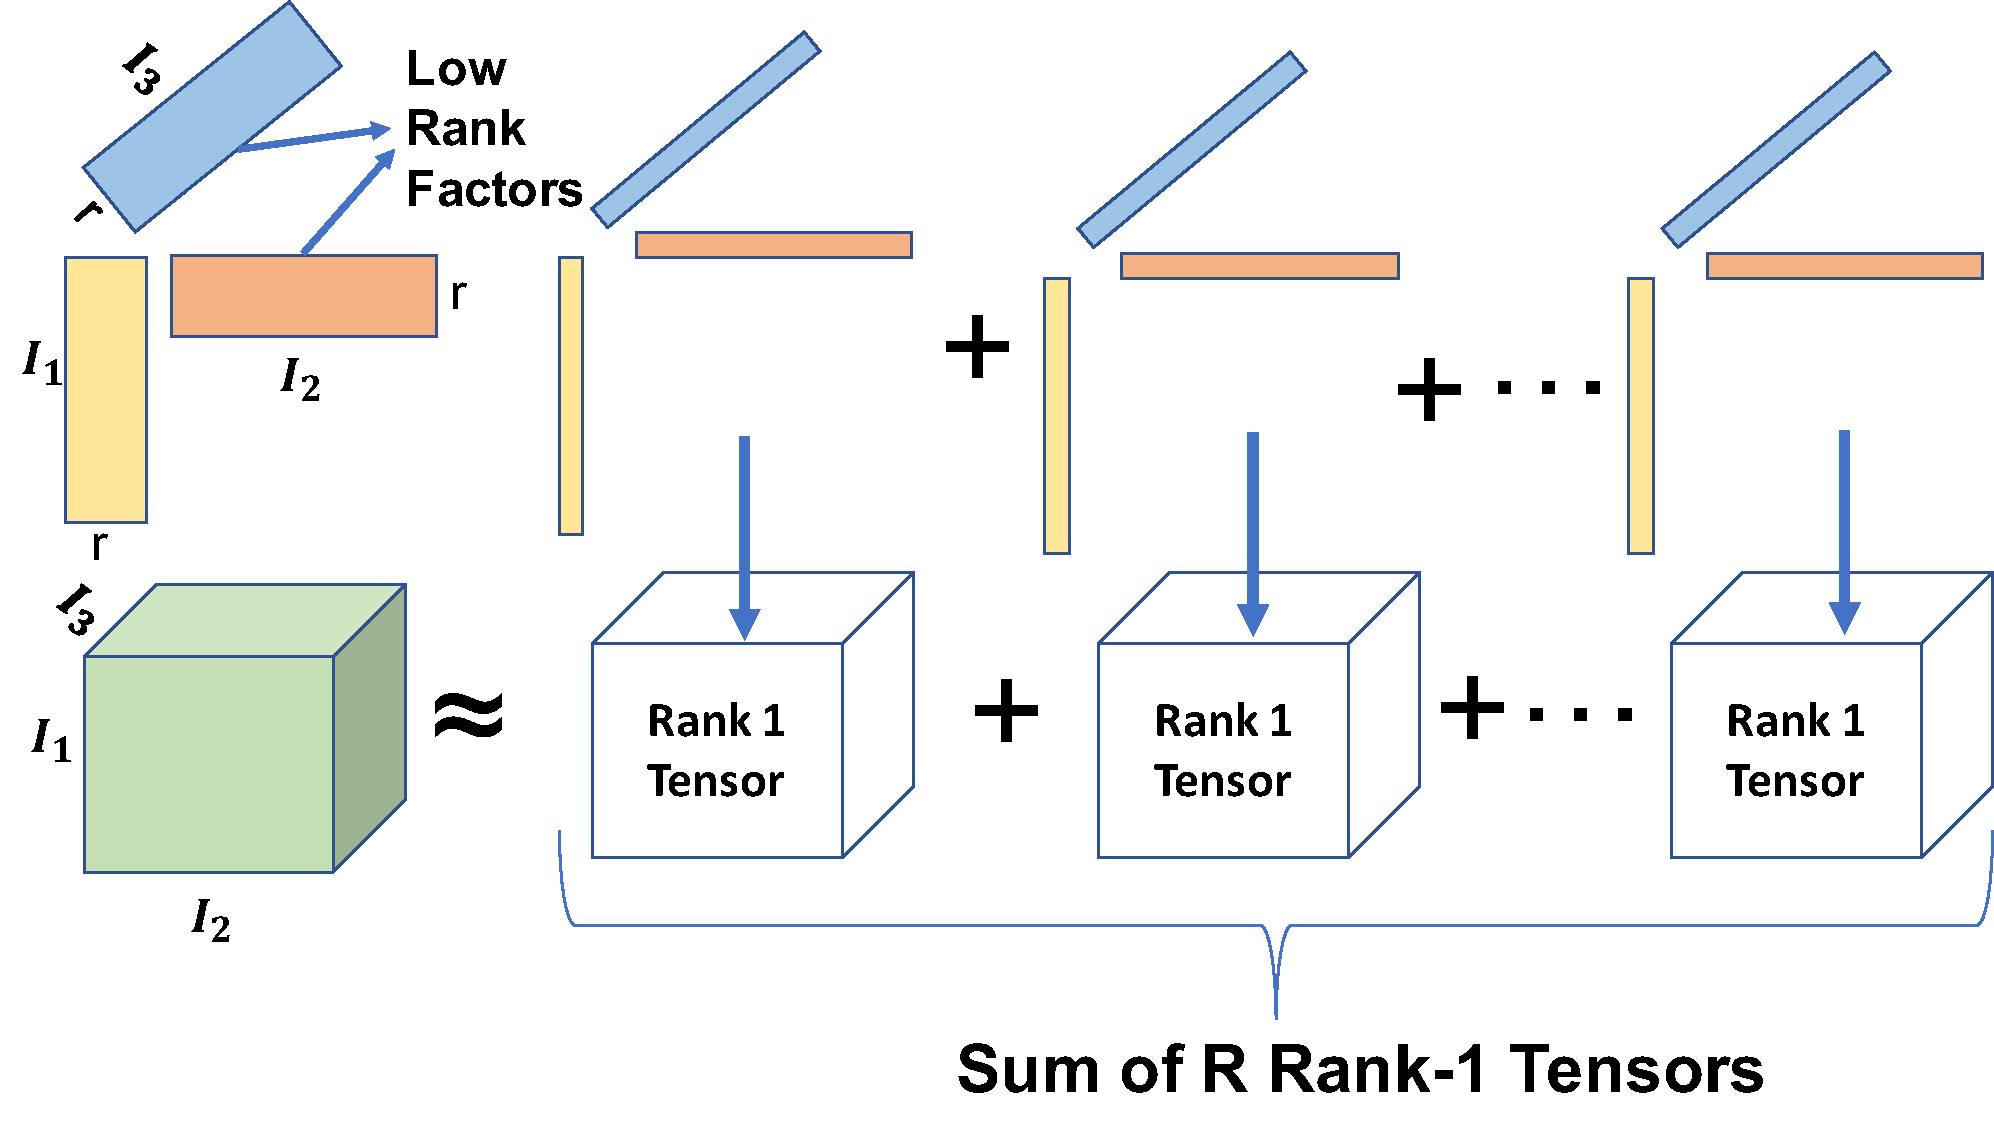
\includegraphics[width=3in, height=1.5in]{fig/cpdecomposition.pdf}
%\caption{CP Decomposition}
%\label{fig:cpdecomposition}
%\end{center}
%\end{figure}


To aid in interpretability, domain-specific constraints are often imposed on the computed factors.
We focus in this paper on dense tensors (when nearly all of the tensor entries are nonzero) and on constraining solutions to have nonnegative entries, which is useful when the tensor data itself is nonnegative. Formally, NNCP can be defined as
\SplitN{\label{eqn:nncp}}{
 \min_{\HH^{(i)} \geq 0} & \| \TA - \sum_{r=1}^R \Mn{H}{1}(:,r) \circ \cdots \circ \Mn{H}{N}(:,r) \|^2
}
where $\Mn{H}{1}(:,i) \circ \cdots \circ \Mn{H}{N}(:,i)$ is the outer product of the $i^{th}$ vector from all the $N$ factors that yields a rank one tensor $\T{M}$ and $\sum_{r=1}^R \Mn{H}{1}(:,r) \circ \cdots \circ \Mn{H}{N}(:,r)$ results in a sum of $R$ rank one tensors that will be of the same dimension as the input tensor $\TA$. 
For example, in imaging and microscopy applications, tensor values often correspond to intensities, and NNCP can be used to cluster and analyze the data in a lower-dimensional space \cite{JC+16}.
In this work, we consider two such applications: a series of time-lapse hyperspectral images \cite{FAN16} and a dynamic functional correlation data set generated from functional magnetic resonance images of human brains \cite{VEU+12}.

One approach to handling multidimensional data is to ``matricize'' it, combining sets of modes to reshape the data into a matrix, so that standard matrix  methods like principal component analysis or nonnegative matrix factorization can be applied.
While this approach can be effective in certain cases, reshaping the data destroys multidimensional relationships among entries that the matrix methods cannot recover.
By maintaining the tensor structure of the data, the low-rank representations preserve these relationships, often producing better and more interpretable results.

However, tensor methods are more complicated both mathematically and computationally.
The kernel computations within standard algorithms for computing NNCP can be formulated as matrix computations, but the complicated layout of tensors in memory prevents the straightforward use of BLAS and LAPACK libraries.
In particular, the matrix formulation of subcomputations involve different views of the tensor data, so no single layout yields a column- or row-major matrix layout for all subcomputations.
Likewise, the parallelization approach for tensor methods is not a straightforward application of parallel matrix computation algorithms.

In developing an efficient parallel algorithm for computing a NNCP of a dense tensor, the key is to parallelize the bottleneck computation known as Matricized-Tensor Times Khatri-Rao Product (MTTKRP), which is performed repeatedly for each mode of the tensor.
The parallelization must load balance the computation, minimize communication across processors, and distribute the results so that the rest of the computation can be performed independently.
In our algorithm, not only do we load balance the computation, but we also compute and store temporary values that can be used across MTTKRPs of different modes using a technique known as dimension trees, significantly reducing the computational cost compared to standard approaches.
Our parallelization strategy also avoids communicating tensor entries and minimizes the communication of factor matrix entries, helping the algorithm to remain computation bound and scalable to high core counts.

As we detail in the related work, the general techniques for reducing computation and communication are not new.
The recomputation avoidance was proposed in a sequential algorithm \cite{PTC13a}, and the parallelization scheme was proposed and analyzed for general tensors \cite{BKR17-TR} and the algorithm was implemented for 3D tensors \cite{LK+17b}.
The main contribution of this paper is the combination and implementation of these ideas for general $N$D tensors, and we demonstrate superior performance to the existing implementation for 3D tensors \cite{LK+17b}.

We summarize our main contributions as follows:
\begin{itemize}
		\item we present a computation- and communication-efficient algorithm for NNCP with detailed cost analysis,
		\item our algorithm is designed for general $N$-way tensors,
		\item we demonstrate a performance improvement of up to $2.2\times$ over the existing state-of-the-art parallel software on 3D tensors,
		\item we demonstrate efficient parallel scaling of up to $253\times$ on $512$ cores.
\end{itemize}

% !TEX root = paper.tex

\section{Preliminaries} 
\label{sec:prelims}

\subsection{Notation}

Tensors will be denoted using Euler script (e.g., $\T{T}$), 
matrices will be denoted with uppercase boldface (e.g., $\M{M}$), vectors will be denoted with lowercase boldface  
(e.g., $\V{v}$), and scalars will not be boldface (e.g., $s$). 
We use Matlab style notation to index into tensors, matrices, and vectors, and we use 1-indexing. 
For example, $\M{M}(:,c)$ gives the $c$th column of the matrix M.

We use $\circ$ to denote the outer product of two or more vectors.
The Hadamard product is the element-wise matrix product and will be denoted using $\Hada$. 
The Khatri-Rao product, abbreviated KRP, will be denoted with $\Khat$. 
Given matrices $\M{A}$ and $\M{B}$ that are $I_{A} \times R$ and $I_{B} \times R$, the KRP $\M{K} = \M{A} \Khat \M{B}$ is $I_{A}I_{B} \times R$. 
It can be thought of as a row-wise Hadamard product, where $\M{K}(i+I_{A}(j{-}1),:) = \M{A}(i,:) \Hada \M{B}(j,:)$, or a column-wise Kronecker product, where $\M{K}(,c) =  \M{A}(:,c) \Kron \M{B}(:,c)$.

The CP decomposition of a tensor (also referred to as the CANDECOMP/PARAFAC or canonical polyadic decomposition) is a low-rank approximation of a tensor, where the approximation is a sum of rank-one tensors and each rank-one tensor is the outer product of vectors.
We use the notation
$$\TA \approx \CP = \sum_{r=1}^R \Mn{H}{1}(:,r) \circ \cdots \circ \Mn{H}{N}(:,r)$$
to represent a rank-$R$ CP model, where $\Mn{H}{n}$ is called a factor matrix and collects the mode-$n$ vectors of the rank-one tensors as columns.
The columns of the factor matrices are often normalized, with weights collected into an auxiliary vector $\V{\lambda}$ of length $R$; in this case we use the notation $\CPl$.

A Nonnegative CP decomposition (NNCP) constrains the factor matrices to have nonnegative values.
In this work, we are interested in NNCP models that are good approximations to $\TA$ in the least squares sense.
That is, we seek to minimize $\|\TA-\CPl\|$, where the tensor norm is a generalization of the matrix Frobenius or vector 2-norm, the square root of the sum of the squares of the entries.

The $n$th mode matricized tensor denoted by $\M{A}_{(n)}$ is a $I_n\times I/I_n$ matrix formed by organizing the $n$th mode fibers of a tensor $\T{X}$ with dimensions $I_{1} \times ... \times I_{N}$ into the columns of a matrix. 
The Matricized Tensor Times Khatri Rao Product or MTTKRP will be central to this work and takes the form $\Mn{M}{n} = \Mz{A}{n}( \Mn{H}{N} \Khat \cdots \Khat \Mn{H}{n+1} \Khat \Mn{H}{n-1} \Khat  \cdots \Khat \Mn{H}{1})$. 

\subsection {Block Coordinate Descent for NNCP}

While there are multiple optimization methods to compute NNCP, we will focus on a class of methods that use Block Coordinate Descent (BCD), which is also known as the nonlinear Gauss-Seidel method \cite{Bertsekas1999}.
In BCD, the variables are partitioned into blocks, and each variable block is cyclically updated with all other blocks fixed.
For details on the convergence properties and comparisons of BCD methods for nonnegative matrix and tensor decomposition problems, see \cite{KHP2014}.
We consider BCD methods for NNCP that choose the factor matrices as the blocks, which is also often referred to as Alternating Least Squares.
In this case, every subproblem is a linear nonnegative least squares problem.

\Cref{alg:nncp} shows the pseudocode for BCD applied to NNCP.
\Cref{line:MTTKRP,line:GH,line:Gn} compute matrices involved in the gradients of the subproblem objective functions, and \cref{line:NLS} uses those matrices to update the current factor matrix.

The NLS-Update in \cref{line:NLS} can be implemented in different ways.
In a faithful BCD algorithm, the subproblems are solved exactly; in this case, the subproblem is a nonnegative linear least squares problem, which is convex.
We use the Block Principal Pivoting (BPP) method \cite{KP2011,KHP2014}, which is an active-set-like method, to solve the subproblem exactly.
BPP is an active-set-like method for solving the NLS subproblems in Eq. \eqref{eqn:single NLS}.

However, as discussed in \cite{KBP2018} for the matrix case, there are other reasonable alternatives to updating the factor matrix without solving the subproblem exactly.
For example, we can more efficiently update individual columns of the factor matrix as is done in the Hierarchical Alternating Least Squares (HALS) method \cite{CP2009}.
In this case, the update rule is 
$$\Mn{H}{n}(:,r) \leftarrow \lt[ \Mn{H}{n}(:,r) + \Mn{M}{n}(:,r) - (\Mn{H}{n} \Mn{S}{n})(:,r)  \rt]_+$$
which involves the same matrices $\Mn{M}{n}$ and $\Mn{S}{n}$ as BPP.
Other possible BCD methods include Alternating Optimization and Alternating Direction Method of Multipliers (AO-ADMM) \cite{HSL2015, SBK2017} and Nestrov-based algorithms \cite{LKLHS2017}.
The parallel algorithm presented in this paper is generally agnostic to the approach used to solve the nonnegative least squares subproblems, as all these methods are bottlenecked by the subroutine they have in common, the MTTKRP. 


%In this section, we will see relevant foundation for using  this
%framework.  The explanation of this section is mainly motivated out of
%Kim, He and Park \cite{KHP2014}. Consider a constrained non-linear optimization problem
%as follows:
%\begin{gather}
%\min f(x)\:\mbox{ subject to }\:x \in\mathcal{X},\label{eq:general_nonlinear}
%\end{gather}
%Here,  $\mathcal{X}$ is a closed convex subset of $\mathbb{R}^{n}$.
%An important assumption to be exploited in the BCD method is that
%the set $\mathcal{X}$ is represented by a Cartesian product:
%\begin{equation}
%\mathcal{X}=\mathcal{X}_{1}\times\cdots\times\mathcal{X}_{m},\label{eq:bcd-cartesian-product}
%\end{equation}
%where $\mathcal{X}_{j}$, $j=1,\cdots,m$, is a closed convex subset
%of $\mathbb{R}^{N_{j}}$, satisfying $n=\sum_{j=1}^{m}N_{j}$.
%Accordingly, the vector $\mathbf{x}$ is partitioned as
%$\mathbf{x}=(\mathbf{x}_{1},\cdots,\mathbf{x}_{m})$ so that
%$\mathbf{x}_{j}\in\mathcal{X}_{j}$ for $j=1,\cdots,m$. The BCD
%method solves for $\mathbf{x}_{j}$ by fixing all other subvectors of
%$\mathbf{x}$ in a cyclic manner. That is, if
%$\mathbf{x}^{(i)}=(\mathbf{x}_{1}^{(i)},\cdots,\mathbf{x}_{m}^{(i)})$
%is given as the current iterate at the $i^{th}$ step, the algorithm
%generates the next iterate
%$\mathbf{x}^{(i+1)}=(\mathbf{x}_{1}^{(i+1)},\cdots,\mathbf{x}_{m}^{(i+1)})$
%block by block, according to the solution of the following
%subproblem:
%\begin{equation}
%\mathbf{x}_{j}^{(k+1)}\leftarrow\underset{\mathbf{\xi}\in\mathcal{X}_{j}}{\text{argmin}}
%f(\mathbf{x}_{1}^{(k+1)},\cdots,\mathbf{x}_{j-1}^{(k+1)},\mathbf{\xi},\mathbf{x}_{j+1}^{(k)},\cdots,\mathbf{x}_{m}^{(k)}).\label{eq:bcd-method}
%\end{equation}
%Also known as a \textit{non-linear Gauss-Seidel}
%method~\cite{Bertsekas1999}, this algorithm updates one block each
%time, always using the most recently updated values of other blocks
%$\mathbf{x}_{\tilde{j}},\tilde{j}\ne j$. This is important since it
%ensures that after each update, the objective function value does
%not increase. For a sequence $\left\lbrace
%\mathbf{x}^{(i)}\right\rbrace $ where each $\mathbf{x}^{(i)}$ is
%generated by the BCD method, the following property holds.
%\begin{theorem}
%\label{thm:bcd}
%Suppose $f$ is continuously differentiable in $\mathcal{X}=\mathcal{X}_{1}\times\dots\times\mathcal{X}_{m}$,
%where $\mathcal{X}_{j}$, $j=1,\cdots,m$, are closed convex sets.
%Furthermore, suppose that for all $j$ and $i$, the minimum of
%\[
%\min_{\mathbf{\mathbf{\xi}}\in\mathcal{X}_{j}}f(\mathbf{x}_{1}^{(k+1)},\cdots,\mathbf{x}_{j-1}^{(k+1)},\mathbf{\xi},\mathbf{x}_{j+1}^{(k)},\cdots,\mathbf{x}_{m}^{(k)})
%\]
%is uniquely attained. Let $\left\lbrace
%\mathbf{x}^{(i)}\right\rbrace $ be the sequence generated by the
%block coordinate descent method as in Eq.~\eqref{eq:bcd-method}.
%Then, every limit point of $\left\lbrace
%\mathbf{x}^{(i)}\right\rbrace $ is a stationary point. The
%uniqueness of the minimum is not required for the case when  $m=2$
%\cite{GS2000}.
%\end{theorem}
%
%The proof of this theorem for an arbitrary number of blocks is shown
%in Bertsekas~\cite{Bertsekas1999}.
%For a non-convex optimization problem, most algorithms only guarantee
%the stationarity of a limit point \cite{Lin2007}.
%
%When applying the BCD method to a constrained non-linear programming
%problem, we have to ensure the following (a) it is critical to wisely choose a partition of
%$\mathcal{X}$, whose Cartesian product constitutes $\mathcal{X}$. 
%(b)  the dependency among the subproblems -- independent blocks can be 
%computed simultaneously  (c) when updating a block, ensure we are 
%using the most recent other blocks and (d) importantly, every block
%must be solved optimally. Every NTF variant will have different the partition
%scheme for blocks with natural partition such as scalar \cite{SL2001}, vector \cite{CP2009} and matrix \cite{KP2011}. 
%Also, the update equation for determining the optimal block given
%other blocks such as projected gradient, block principal pivoting \cite{KP2011}  etc. 
%A detailed discussion of equivalences and comparison of different NMF and NTF algorithm
%is presented at \cite{KHP2014}. 

\begin{algorithm}
%\caption{$(\CPl,\epsilon) = \text{NNCP}(\TA,k)$}
\caption{$\CP = \text{NNCP}(\TA,k)$}
\label{alg:nncp}
\begin{algorithmic}[1]
\Require $\TA$ is $I_1\times \cdots \times I_N$ tensor, $k$ is approximation rank
\State \Comment{Initialize data}
%\State $\alpha = \|\TA\|^2$
\For{$n=2$ to $N$}
	\State Initialize $\Mn{H}{n}$ 
	\State $\Mn{G}{n} = \MnTra{H}{n}\Mn{H}{n}$
\EndFor
\State \Comment{Compute NNCP approximation}
\While{not converged}
	\State \Comment{Perform outer iteration of BCD}
	\For{$n=1$ to $N$}
	\State \Comment{Compute new factor matrix in $n$th mode}
	\State $\Mn{M}{n} = \text{MTTKRP}(\TA,\{\Mn{H}{i}\},n)$
		\label{line:MTTKRP}
	\State $\Mn{S}{n} = \Mn{G}{1} \Hada \cdots \Hada \Mn{G}{n-1} \Hada \Mn{G}{n+1} \Hada \cdots \Hada \Mn{G}{N}$
		\label{line:GH}
	\State $\Mn{H}{n} = \text{NLS-Update}(\Mn{S}{n},\Mn{M}{n})$
		\label{line:NLS}
%	\State $\Mn[\hat]{H}{n} = \text{NLS-Update}(\Mn{S}{n},\Mn{M}{n})$
%	\State \Comment{Normalize columns}
%	\State $\V{\lambda} = \text{Col-Norms}(\Mn[\hat]{H}{n})$
%	\State $\Mn{H}{n} = \text{Col-Scale}(\Mn[\hat]{H}{n},\V{\lambda})$
%	\State \Comment{Organize data for later modes}
	\State $\Mn{G}{n} = \MnTra{H}{n}\Mn{H}{n}$
		\label{line:Gn}
	\EndFor
%	\State \Comment{Compute relative error $\epsilon$ from mode-$N$ matrices}
%	\State $\beta = \langle \Mn{M}{N},\Mn[\hat]{H}{N} \rangle$
%	\State $\gamma = \V{\lambda}^\Tra (\Mn{S}{N} \Hada \Mn{G}{N}) \V{\lambda}$
%	\State $\epsilon = \sqrt{(\alpha-2\beta+\gamma)/\alpha}$ 
\EndWhile
%\Ensure $\|\TA - \dsquare{\V{\lambda}; \Mn{H}{1},\dots,\Mn{H}{N}}\| /\|\TA\| = \epsilon$
\Ensure $\TA \approx \CP$
\end{algorithmic}
\end{algorithm}

%\subsubsection{Hierarchical Alternating Least Squares (HALS)}
%\label{sec:HALS}
%
%In the case of HALS \cite{CP2009}, updates are performed on individual columns of $\HH$ with all other entries in the factor matrices fixed.
%The update rules \cite[Algorithm 2]{CP2009} can be written in closed form:
%\SplitN{\label{eqn:halsupdate}} {
%\Mn[\hat]{H}{n}_{\V{p}}(:,i) &\leftarrow \lt[ \Mn{H}{n}_{\V{p}}(:,i) + \Mn{M}{n}_{\V{p}}(:,i) - (\Mn{H}{n}_{\V{p}} \Mn{S}{n})(:,i)  \rt]_+\\
%% \ww^i &\leftarrow \lt[ \ww^i + (\AA\HH^T)^i - \WW (\HH \HH^T)^i \rt]_+
%}, 
%
%where, $\Mn{H}{n}_{\V{p}}(:,i) \in \Rn{I_n/P}$ is the $i^{th}$ column of the factor matrix $\Mn{H}{n}_{\V{p}}$.
%Note that the columns of $\Mn{H}{n}_{\V{p}}$ are updated in order, so that the most up-to-date values are always used, and these $nk$ updates can be done in an arbitrary order.  In our case we are updating all the $k$ vectors of a factor $\Mn{H}{n}_{\V{p}}$ one by one. 
%
%\subsection{Alternating Nonnegative Least Squares with Block Principal Pivoting}
%\label{sec:BPP}
%
%Kim and Park \cite{KP2011} first proposed the algorithm and the detail of the BPP algorithm for NTF is explained subsequently in detailed at \cite{KHP2014}. In this paper, we will leverage it to solve the factors $\Mn{H}{n}$. 
%Block Principal Pivoting (BPP) is an active-set-like method for solving the NLS subproblems in Eq. \eqref{eqn:single NLS}.
%\SplitN{\label{eqn:single NLS}}{
%\min_{\xx\geq 0} \|\CC\XX-\BB\|_2.
%}. 
%Kannan, Ballard and Park \cite{KBP2018}, have explained solving the active-set based non-negative least squares 
%using normal equations with $\CC^T\CC$ and $\CC^T\BB$ for determining the non-negative factors of NMF. 
%In our case, $\CC^T\CC$ is $\Mn{S}{n}$ and $\CC^T\BB$ is $\Mn{M}{n}_{\V{p}}$. We use the same implementation
%of BPP from $MPIFAUN$.
%
%Our paper can be extended to other NTF algorithms such as Alternating Optimization and Alternating Direction Method of Multipliers (AO-ADMM) \cite{HSL2015, SBK2017} and Nestrov based updates
%\cite{LKLHS2017} by changing the $Local-NLS-Update$ function of the proposed Algorithm \ref{alg:2D}. 

\subsection{Parallel Computation Model}

%MPI collectives for Prelims
To analyze our algorithms we use the MPI model of distributed-memory parallel computation, where we assume a fully connected network. 
Sending a message of $W$ words from one processor to another costs $\alpha + \beta W$, where $\alpha$ is the latency and $\beta$ to be the per word or bandwidth cost. 
In particular, we will use collective communication over groups of $P$ processors, and we will assume the use of efficient algorithms \cite{TRG05,CH+07}.
In this case, an All-Reduce, which sums data initially distributed across processors and stores the result of size $W$ redundantly on every processor, costs $2\alpha \log P + 2\beta W (P-1)/P$.
An All-Gather collects data initially distributed across processors and stores the union of size $W$ redundantly on all processors and costs $\alpha \log P + \beta W (P-1)/P$.
A Reduce-Scatter sums data initially distributed across processors and partitions the result across processors, which costs $\alpha \log P + \beta W (P-1)/P$, where $W$ is the size of the data that each processor initially stores.
Reduction operations also include a flop cost but we will omit it because it is usually dominated by communication. 



\section{Related Work}\label{sec:related}


In the data mining and machine learning literature there is an overlap between low rank approximations and matrix factorizations due to the nature of applications. 
Despite its name, non-negative matrix ``factorization'' is really a low rank approximation. 
Recently there is a growing interest in collaborative filtering based 
recommender systems. One of the popular techniques
for collaborative filtering is matrix factorization, often with nonnegativity constraints, 
and its implementation is widely available in many
off-the-shelf distributed machine learning libraries
such as GraphLab \cite{low2012}, MLLib \cite{meng2015mllib},
and many others \cite{satish2014,yun2014} as well.
However, we would like to clarify that collaborative
filtering using matrix factorization is a different problem than NMF: 
in the case of collaborative filtering, non-nonzeros in the matrix 
are considered to be missing entries, while in the case of NMF, non-nonzeros in the matrix correspond to true zero values.
 
There are several recent distributed NMF algorithms in the literature \cite{liao2014cloudnmf,Faloutsos2014,Yin2014,liu2010distributed}. 
Liu et al.\ propose running Multiplicative Update (MU) for KL divergence, squared loss, and ``exponential'' loss functions \cite{liu2010distributed}. 
Matrix multiplication, element-wise multiplication, and element-wise division are the building blocks of the MU algorithm. 
The authors discuss performing these matrix operations effectively in Hadoop for sparse matrices. 
Using similar approaches, Liao et al.\ implement an open source Hadoop-based MU algorithm and study its scalability on large-scale biological data sets \cite{liao2014cloudnmf}. 
Also, Yin, Gao, and Zhang present a scalable NMF that can perform frequent updates, which aim to use the most recently updated data \cite{Yin2014}. 
Similarly Faloutsos et al.\ propose a distributed, scalable method for decomposing matrices, tensors, and coupled data sets through stochastic gradient descent on a variety of objective functions \cite{Faloutsos2014}. 
The authors also provide an implementation that can enforce non-negative constraints on the factor matrices. 
All of these works use Hadoop to implement their algorithms.

We emphasize that our MPI-based approach has several advantages over Hadoop-based approaches:
\begin{itemize}
	\item efficiency -- our approach maintains data in memory, never communicating the data matrix, while Hadoop-based approaches must read/write data to/from disk and involves global shuffles of data matrix entries;
	\item generality -- our approach is well-designed for both dense and sparse data matrices, whereas Hadoop-based approaches generally require sparse inputs;
	\item privacy -- our approach allows processors to collaborate on computing an approximation without ever sharing their local input data (important for applications involving sensitive data, such as electronic health records), while Hadoop requires the user to relinquish control of data placement.
\end{itemize}

We note that Spark \cite{ZCFSS10} is a popular big-data processing infrastructure that is generally more efficient for iterative algorithms such as NMF than Hadoop, as it maintains data in memory and avoids file system I/O.
Even with a Spark implementation of previously proposed Hadoop-based NMF algorithm, we expect performance to suffer from expensive communication of input matrix entries, and Spark will not overcome the shortcomings of generality and privacy of the previous algorithms.
Although Spark has collaborative filtering libraries such as MLlib \cite{meng2015mllib}, which use matrix factorization and can impose non-negativity constraints, none of them implement pure NMF, and so we do not have a direct comparison against NMF running on Spark.
As mentioned above, the problem of collaborative filtering is different from NMF, and therefore different computations are performed at each iteration.

%Apart from the distributed implementation for NMF, we would also like to highlight few recent theoretical highlights with NMF under some mild assumptions. 
%Arora, Ge, Kannan and Moitra \cite{AGKM2012}, proposed a initial polynomial time running algorithm for topic modeling with NMF when there exists  anchor words, words that appear (with positive probability) in only one topic. 
%Later, Huang, Sidiropoulos and Swami \cite{HSS2016} improved up on these results under milder conditions using second-order moments. 
%The uniqueness of NMF has been of interest to the community and some recent results for both symmetric and non-symmetric matrices have been obtained using a geometrical point of view in \cite{HSS2013, HSS2014}. 

Fairbanks et al. \cite{Fairbanks2015} present a parallel NMF algorithm designed for multicore machines.  
To demonstrate the importance of minimizing communication, we consider this approach to parallelizing an alternating-updating NMF algorithm in distributed memory (see Section \ref{sec:naive}).
While this naive algorithm exploits the natural parallelism available within the alternating iterations (the fact that rows of $\WW$ and columns of $\HH$ can be computed independently), it performs more communication than necessary to set up the independent problems.
We compare the performance of this algorithm with our proposed approach to demonstrate the importance of designing algorithms to minimize communication; that is, simply parallelizing the computation is not sufficient for satisfactory performance and parallel scalability.

Apart from distributed NMF algorithms using Hadoop and multicores, there are also implementations of the
MU algorithm in a distributed memory setting using X10 \cite{Grove2014} and on a GPU \cite{mejia2015nmf}. 



% !TEX root = paper.tex

\section{Algorithm} 
\label{sec:algorithm}

\subsection{Dimension Trees}
\label{sec:dimtrees}

An important optimization of the CP-ALS algorithm is to re-use temporary values across inner iterations \cite{PTC13a,KU16-TR,LCPSV17,Kaya17}.
To illustrate the idea, consider a 3-way tensor $\T{X}$ approximated by $\dsquare{\M{U},\M{V},\M{W}}$ and the two MTTKRP computations $\Mn{M}{1}=\underline{\Mz{X}{1}(\M{W}}\Khat\M{V})$ and $\Mn{M}{2}=\underline{\Mz{X}{2}(\M{W}}\Khat\M{U})$ used to update factor matrices $\M{U}$ and $\M{V}$, respectively.
The underlined parts of the expressions correspond to the shared dependence of the outputs on the tensor $\T{X}$ and the third factor matrix $\M{W}$.
Indeed, a temporary quantity, which we refer to as a \emph{partial MTTKRP}, can be computed and re-used across the two MTTKRP expressions.
We refer to the computation that combines the temporary quantity with the other factor matrix to complete the MTTKRP computation as a multi-tensor-times-vector or \emph{multi-TTV}, as it consists of multiple operations that multiply a tensor times a set of vectors, each corresponding to a different mode.
%This terminology was used in \cite{HBJT18}.

To understand the steps of the partial MTTKRP and multi-TTV operations in more detail, we consider $\T{X}$ to be $I\times J\times K$ and $\M{U}$, $\M{V}$, and $\M{W}$ to have $R$ columns.
Then 
\begin{equation*}
\MnE{M}{1}{ir} = \sum_{i,j} \TE{X}{ijk} \ME{V}{jr} \ME{W}{kr} 
= \sum_{j} \ME{V}{jr} \sum_k \TE{X}{ijk} \ME{W}{kr} 
= \sum_{j} \ME{V}{jr} \TE{T}{ijr},
\end{equation*}
where $\T{T}$ is an $I\times J\times R$ tensor that is the result of a partial MTTKRP between tensor $\T{X}$ and the single factor matrix $W$.
Likewise,
\begin{equation*}
\MnE{M}{2}{jr} = \sum_{i,k} \TE{X}{ijk} \ME{U}{ir} \ME{W}{kr} 
= \sum_{i} \ME{U}{ir} \sum_k \TE{X}{ijk} \ME{W}{kr} 
= \sum_{i} \ME{U}{ir} \TE{T}{ijr},
\end{equation*}
and we see that the temporary tensor $\T{T}$ can be re-used.
From these expressions, we can also see that computing $\T{T}$ (a partial MTTKRP) corresponds to a matrix-matrix multiplication, and computing each of $\Mn{M}{1}$ and $\Mn{M}{2}$ from $\T{T}$ (a multi-TTV) corresponds to $R$ independent matrix-vector multiplications.
In this case, we compute $\Mn{M}{3}$ using a full MTTKRP.

For a larger number of modes, a more general approach can organize the temporary quantities to be used over a maximal number of MTTKRPs.
The general approach can yield significant benefit, decreasing the computation by a factor of approximately $N/2$ for dense $N$-way tensors.
The idea is introduced in \cite{PTC13a}, but we adopt the terminology and notation of \emph{dimension trees} used for sparse tensors in \cite{KU16-TR,Kaya17}.
In this notation, the root node is labeled $\{1,\dots,N\}$ and corresponds to the original tensor, a leaf is labeled $\{n\}$ and corresponds to the $n$th MTTKRP result, and an internal node is labeled by a set of modes $\{i,\dots,j\}$ and corresponds to a temporary tensor whose values contribute to the MTTKRP results of modes $i,\dots,j$.

\begin{figure}
% !TEX root = ../paper.tex

\begin{center}
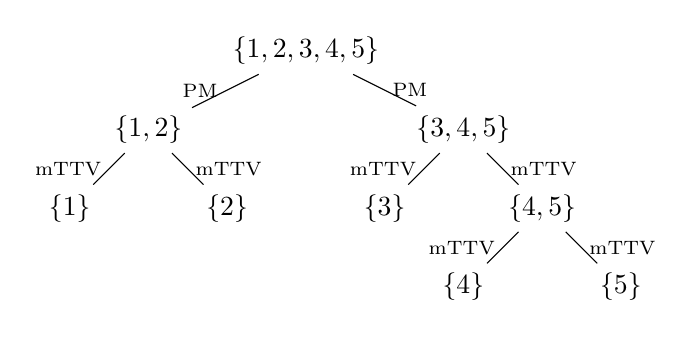
\begin{tikzpicture}

\node (12345) at (4,2) {$\{1,2,3,4,5\}$};
\node (12) at (2,1) {$\{1,2\}$};
\node (345) at (6,1) {$\{3,4,5\}$};
\node (1) at (1,0) {$\{1\}$};
\node (2) at (3,0) {$\{2\}$};
\node (3) at (5,0) {$\{3\}$};
\node (45) at (7,0) {$\{4,5\}$};
\node (4) at (6,-1) {$\{4\}$};
\node (5) at (8,-1) {$\{5\}$};

\scriptsize
\path[draw] (12345) edge [left,align=right] node {PM} (12);
\path[draw] (12345) edge [right,align=left] node {PM} (345);
\path[draw] (12) edge [left,align=right] node {mTTV} (1);
\path[draw] (12) edge [right,align=left] node {mTTV} (2);
\path[draw] (345) edge [left,align=right] node {mTTV} (3);
\path[draw] (345) edge [right,align=left] node {mTTV} (45);
\path[draw] (45) edge [left,align=right] node {mTTV} (4);
\path[draw] (45) edge [right,align=left] node {mTTV} (5);
\normalsize

\end{tikzpicture}
\end{center}
\caption{Dimension tree example for $N=5$. 
The data associated with the root node is the original tensor, the data associated with the leaf nodes are MTTKRP results, and the data associated with internal nodes are temporary tensors.  
Edges labeled with PM correspond to partial MTTKRP computations, and edges labeled with mTTV correspond to multi-TTV computations.}
\label{fig:DT}
\end{figure}

\Cref{fig:DT} illustrates a dimension tree for the case $N=5$.
Various shapes of binary trees are possible \cite{PTC13a,Kaya17}.
For dense tensors, the computational cost is dominated by the root's branches, which correspond to partial MTTKRP computations.
We perform the splitting of modes at the root so that modes are chosen contiguously with the respect to the layout of the tensor entries in memory.
In this way, each partial MTTKRP can be performed via BLAS's GEMM interface without reordering tensor entries in memory.
All other edges in a tree correspond to multi-TTVs and are typically much cheaper.
By organizing the memory layout of temporary quantities, the multi-TTV operations can be performed via a sequence of calls using BLAS's GEMV interface.
By using the BLAS in our implementation, we are able to obtain high performance and on-node parallelism.

\begin{figure}
\subfloat[Partial MTTKRP to compute node $\{3,4,5\}$ from root node $\{1,2,3,4,5\}$, executed via one GEMM call. \label{fig:DT-PM}]{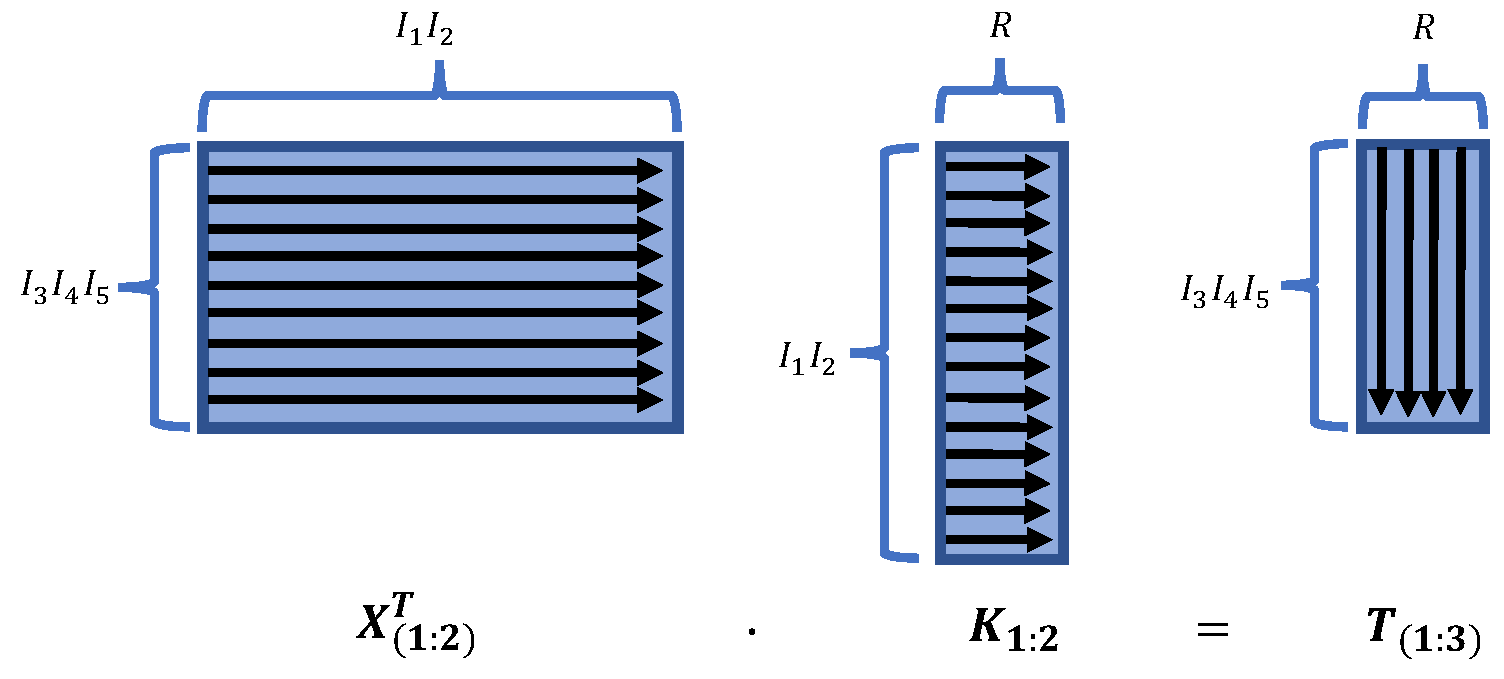
\includegraphics[width=\columnwidth]{fig/PM}} \\
\subfloat[Multi-TTV to compute node $\{3\}$ from node $\{3,4,5\}$, executed via $R$ GEMV calls.  Here $\Mz{T}{1} \lbrack r\rbrack$ refers to the $r$th contiguous block of $\Mz{T}{1}$. \label{fig:DT-mTTV}]{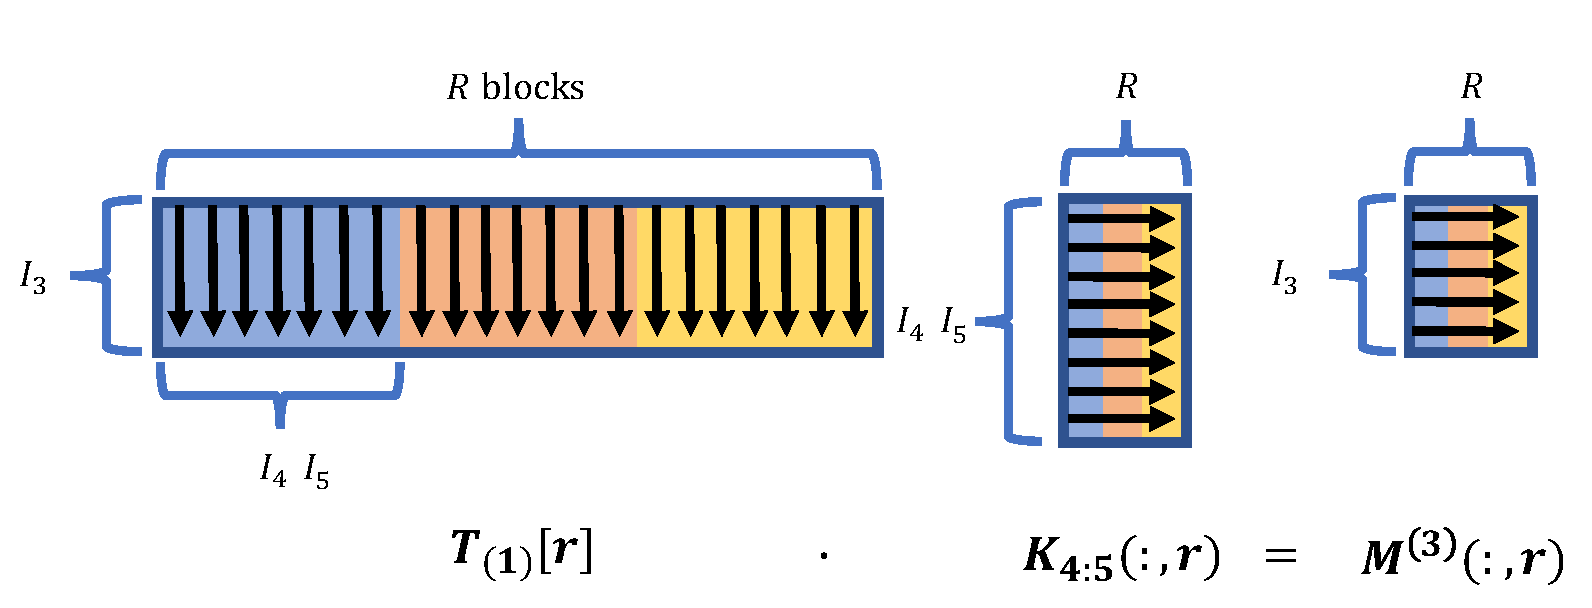
\includegraphics[width=\columnwidth]{fig/mTTV}}
\caption{Data layout and dimensions for two example computations in dimension tree shown in \Cref{fig:DT}.  In this notation, $\Mz{X}{3:5}$ is the matricization of input tensor $\T{X}$ with respect to modes 3 through 5, $\M{K}_{1:2} = \Mn{H}{2} \Khat \Mn{H}{1}$, $\T T$ is the temporary $I_3 \times I_4 \times I_5 \times R$ tensor corresponding to node $\{3,4,5\}$ in the dimension tree, $\M{K}_{4:5} = \Mn{H}{5} \Khat \Mn{H}{4}$, and $\Mn{M}{3}$ is the MTTKRP result for mode 3.}
\label{fig:DTcartoon}
\end{figure}

\Cref{fig:DTcartoon} shows the data layout and dimensions of a partial MTTKRP and a multi-TTV taken from the example dimension tree in \Cref{fig:DT}.
\Cref{fig:DT-PM} shows a partial MTTKRP between the input tensor $\T{X}$ and the Khatri-Rao product of the factor matrices in modes 1 and 2, which produces a temporary tensor $\T{T}$ corresponding to the $\{3,4,5\}$ node in the dimension tree.
The key to efficiency in this computation is that the matricization of $\T{X}$ that assigns modes 1 through 2 to rows and modes 3 through 5 to columns is already column-major in memory.
Thus, we can use the GEMM interface and compute the temporary tensor $\T{T}$ without reordering any tensor entries.
\Cref{fig:DT-mTTV} depicts a multi-TTV that computes the results $\Mn{M}{3}$ from $\T{T}$ and the factor matrices in modes 4 and 5.
Here, the tensor $\T{T}$ is matricized with respect to only its first mode (of dimension $I_3$), but this matricization is also column-major in memory.
We choose the ordering of the modes of $\T{T}$ such that each of $R$ contiguous blocks is used to compute one column of the output matrix via a matrix-vector operation with a corresponding column of the Khati-Rao product of the other factor matrices.

No matter how the dimension tree is designed, the computational cost of each partial MTTKRP is $O(IR)$, where $I$ is the number of tensor entries and $R$ is the rank of the CP decomposition.
This is the same operation count as a full MTTKRP.
The computational cost of a multi-TTV is the number of entries in the temporary tensor, which is the product of a \emph{subset} of the original tensor dimensions multiplied by $R$.
Thus, it is computationally cheaper than the partial MTTKRPs, but it is also memory bandwidth bound.

The other subroutine necessary for implementing the dimension tree approach is the Khatri-Rao product of sets of factor matrices.
We implement the operation as a row-wise Hadamard product of a set of factor matrix rows, and we use OpenMP parallelization to obtain on-node parallelism.
The computational cost of this operation is also typically lower order, but the running time in practice suffers from also being memory bandwidth bound.

\Cref{alg:simpleDT} gives pseudo code for the dimension tree implemented in PLANC. This code follows a dimension tree format which computes MTTKRPS in ascending order, that is 0 to $N$. There is a need for extra storage space to save the results of partial MTTKRPs and multi-TTVs. This is denoted as a tensor $\hat{\T{X}}$. Note that this tensor is always $R \ \times$ a subset of contiguous tensor dimensions. This means that $\hat{\T{X}}$ can always be thought of as a column major matrix with $R$ columns. The multi-TTV operations require that the columns of $\hat{\T{X}}$ be logically reshaped into smaller matrices to perform $R$ matrix vector products. $\hat{\T{X}}^i$ denotes accessing the data which makes up the ith column of $\hat{\T{X}}$. The amount of additional memory needed for $\hat{\T{X}}$  is the size of the larger partial MTTKRP and is $O(I)$ if $R$ is less than the smallest tensor dimension.


\begin{algorithm}
\caption{Simple Dim Tree}
\label{alg:simpleDT}
\begin{algorithmic}
\Require $\T{X}$ is an $N$-way tensor, $n \in [N]$, $s$ split dimension, $n$ loops over $0:N-1$, and projection tensor $\hat{\T{X}}$ for storing intermediate tensor products.
\If{n == 0 or n == N-1}
	\If{n = 0}
		\State $\M{K} \leftarrow (\M{H}^{(s+1)} \bigodot ... \bigodot \M{H}^{(N)}) $
		\State $\hat{\T{X}} \leftarrow \T{X}(0:s,s+1:N) \cdot \M{K}$
		\For{i=1:R}
			\State $\M{M}(:,i) \leftarrow \hat{\T{X}}^i(0,1:s) \cdot (\M{H}^{(1)} \bigodot ... \bigodot \M{H}^{(s)})$
		\EndFor
	\Else % N-1 = n
		\State $\M{K} \leftarrow (\M{H}^{(0)} \bigodot ... \bigodot \M{H}^{(s)})$
		\State $\hat{\T{X}} \leftarrow \Tr{X}(0:s,s+1:N)^\Tra \cdot \M{K}$
		\For{i=1:R}
			\State $\M{M}(:,i) \leftarrow \hat{\T{X}}^i(s+1,s+2:N) \cdot (\M{H}^{(s+2)} \bigodot ... \bigodot \M{H}^{(N)})$
		\EndFor
	\EndIf
\
\Else
	\If{n $\leq$ s}
		\State Y = s
	\Else
		\State Y = N
	\EndIf
	\For{i=1:R}
		\State  $\M{K} \leftarrow \M{H}^{(n-1)}$
		\State $\hat{\T{X}}^i \leftarrow \M{K}_i \cdot \hat{\T{X}}^i(n-1,n:Y)$ % Update to X
	\EndFor
	\For{i=1:R}
		\State  $\M{K} \leftarrow (\M{H}^{(n+1)} \bigodot ... \bigodot \M{H}^{(Y)})$
		\State $\M{M}(:,i) \leftarrow \hat{\T{X}}^i(n,n+1:Y) \cdot \M{K}_i$
	\EndFor
\EndIf
\end{algorithmic}
\end{algorithm}

\subsection{Relative Error Computation}
\label{sec:error}

Given a model $\T{M}=\CP$, we compute the relative error $\|\TA - \T{M}\|/\|\TA\|$ efficiently by using the identity $\|\TA-\T{M}\|^2 = \|\TA\|^2 - 2\langle \TA, \T{M} \rangle + \|\T{M}\|^2.$
The quantity $\|\TA\|$ is fixed, and the other two terms can be computed cheaply given the temporary matrices computed during the course of the BCD algorithm.
The second term can be computed using the identity $\langle \TA, \T{M} \rangle = \langle \Mn{M}{N}, \Mn{H}{N} \rangle$, where $\Mn{M}{N} = \Mz{A}{N} (\Mn{H}{N-1} \Khat \cdots \Khat \Mn{H}{1})$ is the MTTKRP result in the $N$th mode.
The third term can be computed using the identity $\|\T{M}\|^2 = \V{1}^\Tra(\Mn{S}{N} \Hada \MnTra{H}{N} \Mn{H}{N})\V{1}$ where $\Mn{S}{N}=\MnTra{H}{1} \Mn{H}{1} \Hada \cdots \Hada \MnTra{H}{N-1} \Mn{H}{N-1}$.
Both matrices $\Mn{M}{N}$ and $\Mn{S}{N}$ are computed during the course of the BCD algorithm for updating the factor matrix $\Mn{H}{N}$.
The extra computation involved in computing the relative error is negligible.
These identities have been used previously \cite{KB2009,TensorBox,SK16,LKLHS2017}.

\subsection{Parallel Algorithm}

\begin{algorithm}
\caption{$\CP = \text{Par-NNCP}(\TA,R)$}
\label{alg:Par-NNCP-short}
\begin{algorithmic}[1]
\Require $\TA$ is an $I_1\times \cdots \times I_N$ tensor distributed across a $P_1\times \cdots \times P_N$ grid of $P$ processors, so that $\TA_{\V{p}}$ is $(I_1/P_1)\times \cdots \times (I_N/P_N)$ and is owned by processor $\V{p}=(p_1,\dots,p_N)$, $R$ is rank of approximation
\For{$n=2$ to $N$}
	\State Initialize $\Mn{H}{n}_{\V{p}}$ of dimensions $(I_n/P)\times R$ 
	\State $\M[\overline]{G} = \text{Local-SYRK}(\Mn{H}{n}_{\V{p}})$
	\State $\Mn{G}{n} = \text{All-Reduce}(\M[\overline]{G},\textsc{All-Procs})$
	\State $\Mn{H}{n}_{p_n} = \text{All-Gather}(\Mn{H}{n}_{\V{p}},\textsc{Proc-Slice}(n,\VE{p}{n}))$
\EndFor
\State \Comment{Compute NNCP approximation}
\While{not converged}
	\label{line:while}
	\State \Comment{Perform outer iteration of BCD}
	\For{$n=1$ to $N$}
		\label{line:for}
		\State \Comment{Compute new factor matrix in $n$th mode}
		\State $\M[\overline]{M} = \text{Local-MTTKRP}(\TA_{p_1\cdots p_N},\{\Mn{H}{i}_{p_i}\},n)$
			\label{line:locMTTKRP}
		\State $\Mn{M}{n}_{\V{p}} = \text{Reduce-Scatter}(\M[\overline]{M},\textsc{Proc-Slice}(n,\VE{p}{n}))$ 
			\label{line:reduce-scatter}
		\State $\Mn{S}{n} = \Mn{G}{1} \Hada \cdots \Hada \Mn{G}{n-1} \Hada \Mn{G}{n+1} \Hada \cdots \Hada \Mn{G}{N}$
			\label{line:hadamard}
		\State $\Mn{H}{n}_{\V{p}} = \text{Local-NLS-Update}(\Mn{S}{n},\Mn{M}{n}_{\V{p}})$
			\label{line:locNLS}
		\State \Comment{Organize data for later modes}
		\State $\M[\overline]{G} = {\Mn{H}{n}_{\V{p}}}^\Tra\Mn{H}{n}_{\V{p}}$
			\label{line:locSYRK}
		\State $\Mn{G}{n} = \text{All-Reduce}(\M[\overline]{G},\textsc{All-Procs})$
			\label{line:all-reduce}
		\State $\Mn{H}{n}_{p_n} = \text{All-Gather}(\Mn{H}{n}_{\V{p}},\textsc{Proc-Slice}(n,\VE{p}{n}))$
			\label{line:all-gather}
	\EndFor 
		\label{line:endfor}
\EndWhile
	\label{line:endwhile}
\Ensure $\TA \approx \CP$
\Ensure Local matrices: $\Mn{H}{n}_{\V{p}}$ is $(I_n/P)\times R$ and owned by processor $\V{p}=(p_1,\dots,p_N)$, for $1\leq n \leq N$, $\V{\lambda}$ stored redundantly on every processor
\end{algorithmic}
\end{algorithm}

\subsubsection{Algorithm Overview}

The basic sequential algorithm is given in \Cref{alg:nncp}, and the parallel version is given in \Cref{alg:Par-NNCP-short}.
We will refer to both the inner iteration, in which one factor matrix is updated (\cref{line:for} to \cref{line:endfor}), and the outer iteration, in which all factor matrices are updated (\cref{line:while} to \cref{line:endwhile}).
In the parallel algorithm, the processors are organized into a logical multidimensional grid (tensor) with as many modes as the data tensor.
The communication patterns used in the algorithm are all MPI collectives, including All-Reduce, Reduce-Scatter, and All-Gather.
The processor communicators (across which the collectives are performed) include the set of all processors and the sets of processors within the same processor slice.
Processors within a mode-$n$ slice all have the same $n$th coordinate.

The method of enforcing the nonnegativity constraints of the linear least squares solve (or update) generally affects only local computation because each row of a factor matrix can be updated independently.
In our algorithm, each processor solves the linear problem or computes the update for its subset of rows (see \cref{line:locNLS}). 
The most expensive (and most complicated) part of the parallel algorithm is the computation of the MTTKRP, which corresponds to \cref{line:locMTTKRP,line:reduce-scatter,line:all-gather}.

The details that are omitted from this presentation of the algorithm include the normalization of each factor matrix after it is computed and the computation of the residual error at the end of an outer iteration.
The computations do involve both local computation and communication, but their costs are negligible.
A more detailed pseudocode is given in \Cref{alg:Par-NNCP-long}.

% !TEX root = ../paper.tex

\newcommand{\procdim}{3}
\newcommand{\proc}{\draw[black,shift={(-.5,-.5)}] (0,0) grid (\procdim,\procdim);}
\newcommand{\highlight}{gray!75}
\newcommand{\commhighlight}{gray!25}
\newcommand{\parscale}{.46}
\newcommand{\secfaclabel}{$\Mn{M}{2}$}

\newcommand{\parbasepic}{
% highlight one processor's data
% front face
\begin{scope}[canvas is yz plane at x=.5,shift={(1.5,-1.5)}]
	% highlight front face of tensor block
	\draw[fill=\highlight,shift={(0,1)}] (0,0) rectangle (1,1);
	% highlight block of 1st factor matrix
	\draw[fill=\highlight,shift={(-2.5,2-1/3)},xscale=.5] (0,0) rectangle (-1,-1/9);
	% highlight block of 2nd factor matrix
	\draw[shift={(0,-1.5)},yscale=.5] (0,0) rectangle (1/9,-1);
\end{scope}
% right face
\begin{scope}[canvas is zx plane at y=(\procdim-.5),rotate=-90,shift={(-.5,-3)}]
	% highlight front face of tensor block
	\draw[fill=\highlight,shift={(0,2.5)}] (0,0) rectangle (1,1);
	% highlight block of 3rd factor matrix
	\draw[fill=\highlight,yscale=.5] (0,0) rectangle (1/9,-1);
\end{scope}
% top face
\begin{scope}[canvas is yx plane at z=.5,yscale=-1,rotate=0]
	% highlight front face of tensor block
	\draw[fill=\highlight,shift={(1.5,-.5)}] (0,0) rectangle (1,1);
\end{scope}

% draw tensor
% front face
\begin{scope}[canvas is yz plane at x=.5,rotate=-90]
	\proc
\end{scope}
% top face
\begin{scope}[canvas is yx plane at z=.5,yscale=-1,rotate=0]
	\proc
\end{scope}
% right face
\begin{scope}[canvas is zx plane at y=(\procdim-.5),rotate=180]
	\proc
\end{scope}

% draw factor matrices
% front face
\begin{scope}[canvas is yz plane at x=.5,shift={(1.5,-.5)}]
	% draw 1st factor matrix
	\draw[shift={(-2.5,0)},xscale=.5] (0,-2) grid (-1,1);
	\node[draw=none] at (-3.6,-.5) {\Large $\Mn{H}{1}$};
	% draw 2nd factor matrix
	\draw[shift={(0,-2.5)},yscale=.5] (-2,0) grid (1,-1);
	\node[draw=none] at (-.5,-3.5) {\Large \secfaclabel};
\end{scope}
% right face
\begin{scope}[canvas is zx plane at y=(\procdim-.5),rotate=-90,shift={(1.5,-.5)}]
	% draw 2nd factor matrix
	\draw[shift={(0,-2.5)},yscale=.5] (-2,0) grid (1,-1);
	\node[draw=none] at (-.5,-3.5) {\Large $\Mn{H}{3}$};
\end{scope}
}
\begin{figure*}[t]
\centering
  \subfloat[Start $n$th iteration with redundant subset of rows of each input matrix. \label{fig:inner_a}]{% !TEX root = Alg_header.tex

\begin{tikzpicture}[x={(-0.5cm,-0.4cm)}, y={(1cm,0cm)}, z={(0cm,1cm)},every node/.append style={transform shape},scale=\parscale]

% highlight all-gather/reduce-scatter patterns

% local computation
% front face
\begin{scope}[canvas is yz plane at x=.5]
	% highlight block of 1st factor matrix now owned by processor
	\draw[fill=\highlight,shift={(-1,.5)},xscale=.5] (0,0) rectangle (-1,-1);
\end{scope}
% right face
\begin{scope}[canvas is zx plane at y=(\procdim-.5),rotate=-90]
	% highlight block of 3rd factor matrix now owned by processor
	\draw[fill=\highlight,yscale=.5,shift={(-.5,-6)}] (0,0) rectangle (1,-1);
\end{scope}

% front face
\begin{scope}[canvas is yz plane at x=.5]
	% highlight block of 2nd factor matrix contribution computed by processor
	%\draw[fill=\highlight,shift={(1.5,-3)},yscale=.5] (0,0) rectangle (1,-1);
\end{scope}

\parbasepic

\end{tikzpicture}

}  \quad
  \subfloat[Compute local MTTKRP for contribution to output matrix $\Mn{M}{2}$. \label{fig:inner_b}]{% !TEX root = Alg_header.tex

\begin{tikzpicture}[x={(-0.5cm,-0.4cm)}, y={(1cm,0cm)}, z={(0cm,1cm)},every node/.append style={transform shape},scale=\parscale]

% highlight all-gather/reduce-scatter patterns

% local computation
% front face
\begin{scope}[canvas is yz plane at x=.5]
	% highlight block of 1st factor matrix now owned by processor
	\draw[fill=\highlight,shift={(-1,.5)},xscale=.5] (0,0) rectangle (-1,-1);
\end{scope}
% right face
\begin{scope}[canvas is zx plane at y=(\procdim-.5),rotate=-90]
	% highlight block of 3rd factor matrix now owned by processor
	\draw[fill=\highlight,yscale=.5,shift={(-.5,-6)}] (0,0) rectangle (1,-1);
\end{scope}

% front face
\begin{scope}[canvas is yz plane at x=.5]
	% highlight block of 2nd factor matrix contribution computed by processor
	\draw[fill=\highlight,shift={(1.5,-3)},yscale=.5] (0,0) rectangle (1,-1);
\end{scope}

\parbasepic

\end{tikzpicture}

}  \quad
  \subfloat[Reduce-Scatter to compute and distribute rows of $\Mn{M}{2}$. \label{fig:inner_c}]{% !TEX root = Alg_header.tex

\begin{tikzpicture}[x={(-0.5cm,-0.4cm)}, y={(1cm,0cm)}, z={(0cm,1cm)},every node/.append style={transform shape},scale=\parscale]

% highlight all-gather/reduce-scatter patterns
% reduce-scatter in 2nd mode

% front face
\begin{scope}[canvas is yz plane at x=.5]
	% highlight front face of proc comm
	\draw[fill=\commhighlight,shift={(1.5,.5)}] (0,0) rectangle (1,-3);
	% highlight block of 2nd factor matrix involved in reduce scatter
	\draw[fill=\commhighlight,shift={(1.5,-3)},yscale=.5] (0,0) rectangle (1,-1);
	% highlight block of 2nd factor matrix of computed output
	\draw[fill=\highlight,shift={(1.5,-3)},yscale=.5] (0,0) rectangle (1/9,-1);
	% highlight block of 1st factor matrix now owned by processor
	\draw[fill=\highlight,shift={(-1,.5)},xscale=.5] (0,0) rectangle (-1,-1);
\end{scope}
% right face
\begin{scope}[canvas is zx plane at y=(\procdim-.5),rotate=-90]
	% highlight right face of proc comm
	\draw[fill=\commhighlight,shift={(-.5,.5)}] (0,0) rectangle (3,-3);
	% highlight block of 3rd factor matrix now owned by processor
	\draw[fill=\highlight,yscale=.5,shift={(-.5,-6)}] (0,0) rectangle (1,-1);
\end{scope}
% top face
\begin{scope}[canvas is yx plane at z=.5,yscale=-1,rotate=0]
	% highlight top face of proc comm
	\draw[fill=\commhighlight,shift={(1.5,-.5)}] (0,0) rectangle (1,3);
\end{scope}

\parbasepic

\end{tikzpicture}

} \quad
  \subfloat[Compute local NLS update to obtain $\Mn{H}{2}_{\V{p}}$ from $\Mn{M}{2}_{\V{p}}$ (and $\Mn{S}{2}$). \label{fig:inner_d}]{% !TEX root = Alg_header.tex

\renewcommand{\secfaclabel}{$\Mn{H}{2}$}

\begin{tikzpicture}[x={(-0.5cm,-0.4cm)}, y={(1cm,0cm)}, z={(0cm,1cm)},every node/.append style={transform shape},scale=\parscale]

% highlight all-gather/reduce-scatter patterns
% reduce-scatter in 2nd mode

% front face
\begin{scope}[canvas is yz plane at x=.5]
	% highlight front face of proc comm
	%\draw[fill=\commhighlight,shift={(1.5,.5)}] (0,0) rectangle (1,-3);
	% highlight block of 2nd factor matrix involved in reduce scatter
	%\draw[fill=\commhighlight,shift={(1.5,-3)},yscale=.5] (0,0) rectangle (1,-1);
	% highlight block of 2nd factor matrix of computed output
	\draw[fill=\highlight,shift={(1.5,-3)},yscale=.5] (0,0) rectangle (1/9,-1);
	% highlight block of 1st factor matrix now owned by processor
	\draw[fill=\highlight,shift={(-1,.5)},xscale=.5] (0,0) rectangle (-1,-1);
\end{scope}
% right face
\begin{scope}[canvas is zx plane at y=(\procdim-.5),rotate=-90]
	% highlight right face of proc comm
	%\draw[fill=\commhighlight,shift={(-.5,.5)}] (0,0) rectangle (3,-3);
	% highlight block of 3rd factor matrix now owned by processor
	\draw[fill=\highlight,yscale=.5,shift={(-.5,-6)}] (0,0) rectangle (1,-1);
\end{scope}
% top face
\begin{scope}[canvas is yx plane at z=.5,yscale=-1,rotate=0]
	% highlight top face of proc comm
	%\draw[fill=\commhighlight,shift={(1.5,-.5)}] (0,0) rectangle (1,3);
\end{scope}

\parbasepic

\end{tikzpicture}

} \quad
  \subfloat[All-Gather to collect rows of $\Mn{H}{2}$ needed for later inner iterations. \label{fig:inner_e}]{% !TEX root = Alg_header.tex

\renewcommand{\secfaclabel}{$\Mn{H}{2}$}

\begin{tikzpicture}[x={(-0.5cm,-0.4cm)}, y={(1cm,0cm)}, z={(0cm,1cm)},every node/.append style={transform shape},scale=\parscale]

% highlight all-gather/reduce-scatter patterns
% reduce-scatter in 2nd mode

% front face
\begin{scope}[canvas is yz plane at x=.5]
	% highlight front face of proc comm
	\draw[fill=\commhighlight,shift={(1.5,.5)}] (0,0) rectangle (1,-3);
	% highlight block of 2nd factor matrix involved in reduce scatter
	\draw[fill=\highlight,shift={(1.5,-3)},yscale=.5] (0,0) rectangle (1,-1);
	% highlight block of 2nd factor matrix of computed output
	\draw[fill=\highlight,shift={(1.5,-3)},yscale=.5] (0,0) rectangle (1/9,-1);
	% highlight block of 1st factor matrix now owned by processor
	\draw[fill=\highlight,shift={(-1,.5)},xscale=.5] (0,0) rectangle (-1,-1);
\end{scope}
% right face
\begin{scope}[canvas is zx plane at y=(\procdim-.5),rotate=-90]
	% highlight right face of proc comm
	\draw[fill=\commhighlight,shift={(-.5,.5)}] (0,0) rectangle (3,-3);
	% highlight block of 3rd factor matrix now owned by processor
	\draw[fill=\highlight,yscale=.5,shift={(-.5,-6)}] (0,0) rectangle (1,-1);
\end{scope}
% top face
\begin{scope}[canvas is yx plane at z=.5,yscale=-1,rotate=0]
	% highlight top face of proc comm
	\draw[fill=\commhighlight,shift={(1.5,-.5)}] (0,0) rectangle (1,3);
\end{scope}

\parbasepic

\end{tikzpicture}

}
  \caption{Illustration of 2nd inner iteration of Par-NNCP algorithm for 3-way tensor on a $3\times3\times3$ processor grid, showing data distribution, communication, and computation across steps.  Highlighted areas correspond to processor $(1,3,1)$ and its processor slice with which it communicates.  The column normalization and computation of $\Mn{G}{2}$, which involve communication across all processors, is not shown here.}
  \label{fig:inner} 
\end{figure*}

\subsubsection{Data Distribution}
\label{sec:datadist}

Given a logical processor grid of processors $P_1\times \cdots \times P_N$, we distribute the tensor $\TA$ in a block or Cartesian partition.
Each processor owns a local tensor of dimensions $(I_1/P_1)\times \cdots \times (I_N/P_N)$, and only one copy of the tensor is stored.
Locally, the tensor is stored linearly, with entries ordered in a natural mode-descending way that generalizes column-major layout of matrices.
Given a processor $\V{p}=(\VE{p}{1},\dots,\VE{p}{N})$, we denote its local tensor $\TA_{\V{p}}$.

Each factor matrix is distributed across processors in a block row partition, so that each processor owns a subset of the rows.
We use the notation $\Mn{H}{n}_{\V{p}}$, which has dimensions $I_n/P\times R$ to denote the local part of the $n$th factor matrix stored on processor $\V{p}$.
However, we also make use a redundant distribution of the factor matrices across processors, because all processors in a mode-$n$ processor slice need access to the same entries of $\Mn{H}{n}$ to perform their computations.
The notation $\Mn{H}{n}_{\VE{p}{n}}$ denotes the $I_n/P_n\times R$ submatrix of $\Mn{H}{n}$ that is redundantly stored on all processors whose $n$th coordinate is $\VE{p}{n}$ (there are $P/P_n$ such processors).

Other matrices involved in the algorithm include $\Mn{M}{n}_{\V{p}}$, which is the result of the MTTKRP computation and has the same distribution scheme as $\Mn{H}{n}_{\V{p}}$, and $\Mn{G}{n}$, which is the $R\times R$ Gram matrix of the factor matrix $\Mn{H}{n}$ and is stored redundantly on all processors.

\subsubsection{Inner Iteration}

The inner iteration is displayed graphically in \Cref{fig:inner} for a 3-way example and an update of the $2$nd factor matrix.
The main idea is that at the start of the $n$th inner iteration (\Cref{fig:inner_a}), all of the data is in place for each processor to perform a local MTTKRP computation.
This means that all processors in a slice redundantly own the same rows of the corresponding factor matrix (for all modes except $n$).
After the local MTTKRP is computed (\Cref{fig:inner_b}), each processor has computed a contribution to a subset of the rows of the global MTTKRP $\Mn{M}{n}$, but its contribution must be summed up with the contributions of all other processors in its mode-$n$ slice.
This summation is performed with a Reduce-Scatter collective across the mode-$n$ processor slice that achieves a row-wise partition of the result (in \Cref{fig:inner_c}, the light gray shading corresponds to the rows of $\Mn{M}{2}$ to which processor $(1,3,1)$ contributes and the dark gray shading corresponds to the rows it receives as output).
The output distribution of the Reduce-Scatter is designed so that afterwards, the update of the factor matrix in that mode can be performed row-wise in parallel.
Along with $\Mn{S}{n}$, which can be computed locally, each processor updates its own rows of the factor matrix given its rows of the MTTKRP result (\Cref{fig:inner_d}).
The remainder of the inner iteration is preparing and distributing the new factor matrix data for future inner iterations, which includes an All-Gather of the newly computed factor matrix $\Mn{H}{n}$ across mode-$n$ processor slices (\Cref{fig:inner_e}) and recomputing $\Mn{G}{n}={\Mn{H}{n}}^\Tra\Mn{H}{n}$.

\subsubsection{Analysis}

\begin{table*}
\centering
\begin{tabular}{|c|cccc|}
\hline
 & \textbf{Computation} & \textbf{Memory - Local MTTKRP} & \textbf{Communication} & \textbf{Memory - Par.~Algorithm}  \\
\hline
Par-NNCP w/ opt.~proc.~grid & $\frac{IR}{P}$ & $\frac{RI^{1/2}}{P^{1/2}}$ & $\frac{NRI^{1/N}}{P^{1/N}}$ & $\frac{NRI^{1/N}}{P^{1/N}}$  \\
%\hline
Par-NNCP w/ gen.~proc.~grid & $\frac{IR}{P}$ & $\frac{RI^{1/2}}{P^{1/2}}$ & $\mathbf{R\sum_n \frac{I_n}{P_n}}$ & $\mathbf{R\sum_n \frac{I_n}{P_n}}$  \\
%\hline
Par-NNCP w/o dim.~tree opt. & $\mathbf{\frac{NIR}{P}}$ & $\displaystyle \mathbf{\max_n \frac{RI/I_n}{P/P_n}}$  &  $\frac{NRI^{1/N}}{P^{1/N}}$ & $\frac{NRI^{1/N}}{P^{1/N}}$ \\
\hline
\end{tabular}
\smallskip
\caption{Leading-order per-iteration costs in terms of computation (flops), communication (words moved), and memory (words).  We ignore constants but omit big-Oh notation for clarity.  The first line corresponds to \cref{alg:Par-NNCP-short} with an optimal choice of processor grid and applying the dimension tree optimization locally.  The second line corresponds to the changes in communication and memory for a general processor grid.  The third line corresponds to the changes in computation and memory if the dimension tree optimization is not applied.}
\label{tab:costs}
\end{table*}

We will analyze the cost of a single outer iteration.
While the number of outer iterations is sensitive to the NLS method used, the outer iteration time is generally the same across NLS methods.
We summarize the analysis in \Cref{tab:costs}, showing the differences with and without an optimal processor grid and with and without using a dimension tree.

\paragraph{\emph{Computation}}
The local computation occurs at \cref{line:locMTTKRP,line:hadamard,line:locNLS,line:locSYRK}.
The cost of \cref{line:hadamard} is $O(NR^2)$, the cost of \cref{line:locNLS} is $O(R^3I_n/P)$, which is a loose upper bound for BPP and other methods \cite{KBP16}, and the cost of \cref{line:locSYRK} is $O(R(I_n/P)^2)$.
The sum of these three costs across all inner iterations is $O(R^2N^2+(R^3/P)\sum I_n+(R/P^2)\sum I_n^2)$, which is dominated by the cost of the MTTKRP.
When using dimension trees to perform the MTTKRP (\cref{line:locMTTKRP}), we compute the cost amortized over all inner iterations.
In this case, the cost is dominated by the two partial MTTKRP computations (from the root of the tree), which together are $O((R/P) \prod I_n)=O(IR/P)$ and dominate the costs of the multi-TTVs.
We note that this cost involves the product of all the tensor dimensions, which is why it dominates, and we note that it scales linearly with $P$.

\paragraph{\emph{Communication}}
The communication within the inner iteration occurs at \cref{line:reduce-scatter,line:all-reduce,line:all-gather}.
\Cref{line:all-reduce} involves $O(R^2)$ data and a collective across all processors.
\Cref{line:reduce-scatter,line:all-gather} involve $O(I_nR/P_n)$ data across a subset of $P/P_n$ processors.
Thus, the All-Reduce dominates the latency cost and the Reduce-Scatter/All-Gather dominate the bandwidth cost, for a total outer iteration communication cost of $O(R\sum I_n/P_n)$ words and $O(N\log P)$ messages.
If the optimal processor grid can be chosen to minimize communication (assuming $P$ is sufficiently factorable), then the bandwidth cost can achieve a value of $O(NRI^{1/N}/P^{1/N})$ by making the local tensors as cubical as possible.
We note that this cost scales with $P^{1/N}$, which is far from linear scaling.
However, it is proportional to the geometric mean of the tensor dimensions (on the order of one tensor dimension), which is much less than the computation cost dependence on the product of all dimensions.

\paragraph{\emph{Memory}}
The algorithm requires extra local memory to run.
Aside from the memory required to store the local tensor of $O(I/P)$ words and factor matrices of cumulative size $O((R/P)\sum I_n)$, each processor must be able to store a redundant subset of the rows of the factor matrices it needs to perform MTTKRP computations.
This corresponds to storing $P/P_n$ redundant copies of every factor matrix, which results in a local memory requirement of $O(R \sum I_n/P_n)$ for a general processor grid.
The processor grid that minimizes communication also minimizes local memory, and the extra memory requirement can be as low as $O(NRI^{1/N}/P^{1/N})$, which is typically dominated by $O(I/P)$.

The dimension tree algorithm also requires extra temporary memory space, but the space required tends to be much smaller than what is required to store the local tensor.
If the tensor dimensions can be partitioned into two parts with approximately equal geometric means, the extra memory requirement for running a dimension tree is as small as $O(R\sqrt{I/P})$, which is also typically dominated by $O(I/P)$.

\subsection{NLS Algorithms}
This subsection deals with the nonnegative least squares (NLS) solves needed to update the factor at each inner iteration of the algorithm (\cref{line:locNLS} in \Cref{alg:Par-NNCP-short}). The general problem to be solved in each inner iteration is a constrained least squares problem of the form,

\begin{align}
\M{X} \leftarrow \underset{\M{X} \ge \M{0}}{\argmin} \left\lVert \M{A}\M{X} -\M{B}\right\rVert^2_F
\label{eqn:nls}
\end{align}

In the case of updating the local factor matrix $\Mn{H}{n}_{\V{p}}$ we need to solve~\Cref{eqn:nls} with $\M{X} = \Mn{H}{n}_{\V{p}}$, $\M{A} = \Mn{S}{n}$ and $\M{B} = \Mn{M}{n}_{\V{p}}$. Our framework is capable of supporting any alternating-updating NLS solver~\cite{KBP16}. The NLS solvers which fit this framework and are implemented in our software package are Multiplicative Update~\cite{LS99}, Hierarchical Alternating Least Squares~\cite{CP2009}, Block Principal Pivoting~\cite{KP2011}, Alternating Direction Method of Multipliers~\cite{HSL2016} and Nesterov-type algorithm~\cite{LKLHS2017}. We briefly describe the different solvers below. Note that the descriptions are for the general form of the NLS solver as shown in~\Cref{eqn:nls}.


\subsubsection{Multiplicative Update (MU)}
The MU solve is an elementwise operation. The update rule for each element of $\M{X}$ is as follows,
\begin{align}
\M{X}(i,j) \leftarrow \M{X}(i,j)\frac{\M{B}(i,j)}{\left(\M{A}\M{X}\right)(i,j)}
\end{align}
While this rule does not solve~\Cref{eqn:nls} to optimality it ensures a reduction in the objective value from the initial value of $\M{X}$.

\subsubsection{Hierarchical Alternating Least Squares (HALS)}
HALS updates are performed on individual rows of $\M{X}$. The update rule for row $i$ can be written in closed form as,
\begin{align}
\M{X}(i,:) \leftarrow \left[ \M{X}(i,:) + \frac{\M{B}(i,:) - \left(\M{A}(i,:)\M{X}\right)}{\M{A}(i,i)} \right]_+
\end{align}
The rows of $\M{X}$ are updated in order so that the latest values are used in every update step.

\subsubsection{Block Principal Pivoting (BPP)}
BPP is an active-set like method for solving NLS problems. The main subroutine of BPP is the single right hand side version of~\Cref{eqn:nls},
\begin{align}
\V{x} \leftarrow \underset{\V{x} \ge 0}{\argmin} \left\lVert \M{A}\V{x} -\V{b}\right\rVert^2_F
\label{eqn:snls}
\end{align}
The Karash-Kuhn-Tucker (KKT) optimality conditions for~\Cref{eqn:snls} are shown below,
\begin{subequations}
\begin{align}
\V{y} &= \M{A}^\Tra\M{A}\V{x} - \M{A}^\Tra\V{b} \\
\V{y} &\geq \V{0} \\
\V{x} &\geq \V{0} \\
x_i y_i &= 0 \quad \forall i
\end{align}
\label{eqn:bppkkt}
\end{subequations}
The complementary slackness criteria from the KKT conditions forces the support sets, i.e. the non-zero elements, of $\V{x}$ and $\V{y}$ to be disjoint. This makes~\Cref{eqn:bppkkt} an instance of the \emph{Linear Complementarity Problem} which arises frequently in quadratic programming. When $k \ll \min(m.n)$, active-set methods are preferred since they deal with small matrices of size $m \times k$, $n \times k$ and $k \times k$. In the optimal solution, the active-set is the set of indices where $x_i = 0$ and the remaining indices are referred to as the passive set. Once the active-set is found, we can find the optimal solution to~\Cref{eqn:snls} by using solving an unconstrained least squares problem on the passive set of indices. The BPP algorithm attempts to find the active-set by greedily swapping indices between the intermediate active and passive sets until it finds a solution that satisfies the KKT conditions. Kim and Park discuss the method in greater detail in~\cite{KP2011}. The unconstrained least squares is solved using the Normal Equations method in the software though other methods can also be used.

\subsubsection{Alternating Direction Method of Multipliers (ADMM)}
In the ADMM solver the optimization problem~\Cref{eqn:nls} is reformulated by introducing an auxiliary variable $\M{\hat{X}}$ of size $k \times n$,
\begin{align}
\begin{split}
&\underset{\M{X},\M{\hat{X}}}{\min} \quad \frac 1 2 \left\lVert \M{A}\M{\hat{X}} - \M{B}\right\rVert_F^2 + r(\M{X}) \\
&\textnormal{subject to } \M{X} = \M{\hat{X}}^\Tra 
\end{split}
\label{eqn:admmnls}
\end{align}
Here $r(\cdot)$ is the indicator function of $\mathbb{R}_+$. The updates for the ADMM algorithm becomes,
\begin{align}
\begin{split}
\M{\hat{X}} &\leftarrow \left(\M{A}^\Tra\M{A} + \rho\M{I} \right)^{-1}\left(\M{A}^\Tra\M{B} + \rho\left(\M{X} + \M{U}\right)^\Tra\right) \\
\M{X} &\leftarrow \underset{\M{X}}{\argmin}\ r(\M{X}) + \frac{\rho}{2} \left\lVert \M{X} - \M{\hat{X}}^\Tra + \M{U}\right\rVert_F^2 \\
\M{U} &\leftarrow \M{U} + \M{X} - \M{\hat{X}}^\Tra
\end{split}
\end{align}
where $\M{U}$ is the scaled version of the dual variables corresponding to the equality constraints $\M{X} = \M{\hat{X}}^\Tra$ and $\rho$ is a step size specified by the user. The advantage of using ADMM is the clever splitting of the non-negativity constraints into updates of two blocks of variables $\M{X}$ and $\M{\hat{X}}$. This allows for an unconstrained least squares solve for $\M{\hat{X}}$ and element-wise projections onto $\mathbb{R}_+$ for $\M{X}$. One important fact to notice is that the same matrix $\M{A}^\Tra\M{B}$ and matrix inverse $\Br{\M{A}^\Tra\M{A} + \rho \M{I}}^{-1}$ is used for all the updates. We can therefore cache $\M{A}^\Tra\M{B}$ and the Cholesky decomposition of  $\Br{\M{A}^\Tra\M{A} + \rho \M{I}}$ to save some computations. A comprehensive guide to the ADMM method, convergence properties and selection of optimal $\rho$ can be found in~\cite{boyd2011distributed}.

\subsubsection{Nesterov-type algorithm}
The Nesterov-type algorithm in this package was introduced by Liavas et al~\cite{LKLHS2017}. Their method solves a modified version of NLS problem~\Cref{eqn:nls} with the introduction of a proximal term. The proximal term is useful to handle ill-conditioned instances and guarantee strong convexity. The objective function tackled is,
\begin{align}
\underset{\M{X} \ge \M{0}}{\min} f_p(\M{X}) := \frac 1 2 \left\lVert \M{B}^\Tra - \M{X}^\Tra\M{A}^\Tra \right\rVert_F^2 + \frac{\lambda}{2}\left\lVert\M{X} -\M{X_*}\right\rVert_F^2
\label{eqn:nesnls}
\end{align}
The gradient of $f_p$ is given by the expression,
\begin{align}
\nabla f_p(\M{X}) = -(\M{B}^\Tra - \M{X}^\Tra\M{A}^\Tra)\M{A} + \lambda(\M{X}-\M{X_*})
\end{align}
The first order updates to $\M{X}$ are iterative and sketched below. They are repeated until a termination criteria is triggered. Different criteria are discussed in~\cite{LKLHS2017},
\begin{align}
\begin{split}
\M{Y}_{k+1} &\leftarrow \left[ \M{X}_k - \alpha \nabla f_p(\M{X}_k)\right]_+ \\
\M{X}_{k+1} &\leftarrow \M{Y}_{k+1} + \beta \Br{\M{Y}_{k+1} - \M{Y}_k}
\end{split}
\label{eqn:nesupd}
\end{align}
Here $[\cdot]_+$ is the projection operator in to $\mathbb{R}_+$. The selection of hyperparameters $\lambda, \alpha$ and $\beta$ depends on the spectrum of $\M{A}\M{A}^\Tra$ and is necessary for developing an Nesterov-like method for solving~\Cref{eqn:nesnls}. Details of the selection procedure and different cases can be found in the original paper~\cite{LKLHS2017}. In addition to the acceleration performed during each NLS solve~\Cref{eqn:nesupd} we can also perform an acceleration step for every outer iteration in~\Cref{alg:Par-NNCP-short}~\Cref{line:while}. In this step all factor matrices are updated using the previous iterate values till the objective stops decreasing.



% !TEX root = paper.tex

\section{Performance Results} \label{sec:experiments}

% !TEX root = experiments.tex

% macros for plotting
\newcommand{\datafile}{}
\newcommand{\alg}{}
\newcommand{\numiterations}{30}
\newcommand{\minvalue}{1}

% toggles whether or not to plot naive results (if not, the rows of the data file also need to be commented out)
\newif\ifnaive
% toggles ksweep vs scaling plot
\newif\ifksweep
% toggles legend
\newif\iflegend
% toggles y axis label
\newif\ifylabel
% toggles wider plot area
\newif\ifwider
% toggles including liavas results
\newif\ifliavas


\newcommand{\setcolors}{
\pgfplotsset{cycle list={
	red, fill=red \\ 
	blue, fill=blue \\ 
	green, fill=green \\ 
	red, pattern=crosshatch, pattern color=red \\
	green, pattern=crosshatch, pattern color=green \\
	blue, pattern=crosshatch, pattern color=blue \\
}};
}

% set options for grouped bar plot
\newcommand{\breakdownplotoptions}{
	ybar stacked,
	reverse legend,
	bar width=8pt,
	width=9cm, height=3.85cm,
	ylabel={Time (s)}, 
	y label style={yshift=-.5cm},
	ymin=0,
	symbolic x coords={D1,N1,D16,N16,D81,N81,D256,N256},
	xtick=data,
	legend style={at={(0.5,1.3)},anchor=north},
	legend columns=-1,
	reverse legend
}

% stacked bar plot command
\newcommand{\breakdownplot}{
\begin{axis}[\breakdownplotoptions]
	\setcolors
	\addplot table[x=alg-p, y expr=(\thisrow{mttkrp}/(\minvalue*\numiterations))] {\datafile};
	\addplot table[x=alg-p, y expr=(\thisrow{krp}/(\minvalue*\numiterations))] {\datafile};
	\addplot table[x=alg-p, y expr=((\thisrow{allgather}+\thisrow{reducescatter})/(\minvalue*\numiterations))] {\datafile};
	\addplot table[x=alg-p, y expr=((\thisrow{nnls}+\thisrow{gram}+\thisrow{allreduce})/(\minvalue*\numiterations))] {\datafile};
	\addplot table[x=alg-p, y expr=((\thisrow{err_compute}+\thisrow{err_communication})/(\minvalue*\numiterations))] {\datafile};
	\legend{MTTKRP,KRP,Factor Comm,NLS,Error};
\end{axis}
}

% labels for bar groups (manually positioned)
\newcommand{\labels}{
%\node [align=center,text width=3cm] at (1.25cm, -.95cm)   {\ifksweep 10 \else 16 \fi};
%\node [align=center,text width=3cm] at (3cm, -0.95cm)   {\ifksweep 20 \else 96 \fi};
%\node [align=center,text width=3cm] at (4.6cm, -0.95cm)   {\ifksweep 30 \else 384 \fi};
%\node [align=center,text width=3cm] at (6.3cm, -0.95cm) {\ifksweep 40 \else 864 \fi};
%\node [align=center,text width=3cm] at (8.15cm, -0.95cm) {\ifksweep 50 \else 1536 \fi};
\node [align=center,text width=3cm] at (1cm, -1.15cm)   {\ifksweep 10 \else 1 \fi};
\node [align=center,text width=3cm] at (2.4cm, -1.15cm)   {\ifksweep 20 \else 16 \fi};
\node [align=center,text width=3cm] at (3.7cm, -1.15cm)   {\ifksweep 30 \else 81 \fi};
\node [align=center,text width=3cm] at (5.1cm, -1.15cm) {\ifksweep 40 \else 256 \fi};
}

% allows for filtering rows from dat file
\pgfplotsset{
    discard if not/.style 2 args={
        x filter/.append code={
            \edef\tempa{\thisrow{#1}}
            \edef\tempb{#2}
            \ifx\tempa\tempb
            \else
                \def\pgfmathresult{inf}
            \fi
        }
    }
}

% set options for strongscaling plot
\newcommand{\strongscalingplotoptions}{
		log basis y={2},
		log basis x={2},
		\ifliavas
			xlabel=Cores,
		\else
			xlabel=Nodes,
		\fi
		ylabel=Time (s),
		y tick label style={
	        /pgf/number format/.cd,
            	precision=4,
		},
	legend style={draw=none, cells={align=left}, nodes={scale=0.7}}
}

% plot time over p, filtering rows out appropriately
\newcommand{\strongscalingplot}{
\begin{loglogaxis}[\strongscalingplotoptions]
	%\addplot+ [discard if not={alg}{N},thick,mark options={solid},mark=square*] table [x={p}, y={totaltime}] {\datafile};
	\ifliavas
		\addplot+ [discard if not={alg}{DF},thick,mark options={solid},mark=square*] table [x={p}, y expr=(\thisrow{total}/(\minvalue*\numiterations))] {\datafile};
		\addplot+ [discard if not={alg}{NF},thick,mark options={solid},mark=square*] table [x={p}, y expr=(\thisrow{total}/(\minvalue*\numiterations))] {\datafile};
	\else
		\addplot+ [discard if not={alg}{D},thick,mark options={solid},mark=triangle*] table [x={p}, y expr=(\thisrow{total}/(\minvalue*\numiterations))] {\datafile};
		\addplot+ [discard if not={alg}{N},thick,mark options={solid},mark=square*] table [x={p}, y expr=(\thisrow{total}/(\minvalue*\numiterations))] {\datafile};
	\fi
	\ifliavas
		\addplot+ [discard if not={alg}{L},thick,mark options={solid}] table [x={p}, y expr=(\thisrow{total}/(\minvalue*\numiterations))] {\datafile};
		\legend{DimTree,NoDimTree,NbAO-NTF \cite{LK+17b}}
	\else
		\legend{DimTree,NoDimTree,FlatDimTree,FlatNoDimTree};
	\fi
\end{loglogaxis}
}



\subsection{Datasets}

\subsubsection{Hyperspectral Images (HSI)}
For comparison with previous work \cite{LK+17b}, we consider the same 3D hyperspectral imaging dataset called ``Souto\_wood\_pile'' \cite{FAN16}. 
NNCP is often used on HSI data sets for classification and blind source separation of materials with differing spectral signatures.
The hyperspectral datacube has dimensions $1024 \times 1344 \times 33$ and represents a set of 33 grayscale images of size 1344 $\times$ 1024 pixels sampled at wavelengths 400, 410, $\dots$, 720 nm, with each pixel value representing spectral radiance in $W m^{-2} sr^{-1} nm^{-1}$. 
We also consider the Nogueir\'{o} scene dataset, which is a sequence of 9 time-lapse HSI images of the same scene acquired at about 1-hour intervals.
In each scene, hyperspectral images were acquired at about 1-hour intervals. 
Each Nogueir\'{o} scene HSI image has the same properties as the Souto\_wood\_pile data set, so the corresponding tensor has dimensions $1024 \times 1344 \times 33 \times 9$. 

\subsubsection{Dynamic Functional Connectivity (dFC)}
We also consider dynamic functional connectivity datasets that are generated from fMRI images of human brains.
Given a 4D fMRI data set of voxel measurements across multiple timesteps, voxels containing brain data are partitioned into a set of regions of interest (specified using domain-specific knowledge), and a single time-series signal is aggregated for each region of interest.
Then, an instantaneous correlation is computed for each time point and pair of regions, and this process is repeated for a number of subjects.
Computing a CP decomposition of this data helps to discover patterns of brain connectivity among different regions and also differentiate among individuals.
For our representative dFC data set, we consider 246 brain regions, which yields 30{,}012 unique pairs of regions, 1200 times steps, and 500 subjects, or a tensor of dimension $30{,}012\times 1200 \times 500$ \cite{VEU+12,THBGW17}.

\subsubsection{Synthetic}
Our synthetic data sets are constructed from a CP model with an exact low rank with no added noise.
In this case we can confirm that the residual error of our algorithm with a random start converges to zero.
For the purposes of benchmarking, we run a fixed number of iterations of the BCD algorithm rather than using a convergence check.

%For the synthetic datasets, our open source code supports (a) low-rank tensor (b) uniform random and (c) positive shifted normal distribution of $\mathfrak{N}(3,1)$ -- that is change the mean such that all the random numbers are positive. We considered three different synthetic matrices for different cases. For baseline comparison with Liavas \cite{LK+17b}, we considered a three mode 
%uniform of size 1024x1024x1024 on processor grids $2^k \times 2^k \times 2^k$ for $k \in {0,1,2,3}$. We used the uniform five 
%mode synthetic tensor with dimension $64\times 64\times 64\times 64\times 64$ on processor grids 
%$1\times1\times1\times1\times1$, $2\times1\times1\times1\times1$, $\dots$, $2\times2\times2\times2\times2$ for strong scaling 
%experiments.  In the case of weak scaling of four mode synthetic tensors with (D) and without (N) the use of dimension trees.  The 
%tensor and processor grid dimensions are $128k\times 128k\times 128k\times 128k$ and $k\times k\times k\times k$ for $k\in\{1,2,3,4\}$. In all the cases the dimensions were considered such that synthetic tensors can be accommodated even on single node with 64GB for scale up plots. 

\subsection{Machine Details}
The entire experimentation was performed on Eos, a supercomputer at the Oak Ridge Leadership Computing Facility. 
Eos is a 736-node Cray XC30 cluster of Intel Xeon E5-2670 processors with a total of 47.104TB of memory. 
Its compute nodes are organized in blades where each blade contains 4 nodes, and every node has 2 sockets with 8 physical cores and 64GB memory. 
The machine support Intel's hyper-threading (HT), but we restricted it because HT offers minimal improvement for BLAS and LAPACK operations. 
In total, the Eos compute partition contains 11,776 traditional processor cores and our experiments used up to 4,096 cores (35\% of the machine). 

Our objective of the implementation is using open source software as much as possible 
to promote reproducibility and reuse of our code.
%Unlike Liavas \cite{LK+17b} that uses Eigen matrix library \cite{eigenweb}, 
We use Armadillo \cite{sanderson2010} for matrix representation
and operations.  
In Armadillo, the elements of the dense matrix are stored in column major order.
For dense BLAS and LAPACK operations, we linked Armadillo with the default LAPACK/BLAS wrappers from Cray. 
For compiler, we use GNU C++ Compiler (g++ (GCC) 6.3.0) and MPI library is from Cray.  We could also 
compile and run the code in RHEA the commodity cluster from OLCF with entire open source libraries such as OpenBLAS and OpenMPI. 

\subsection{Comparison Implementations}
The implementation proposed by Liavas et al. \cite{LK+17b} is the only publicly available distributed-memory software (of which we are aware) for computing the CP decomposition of dense tensors, with or without constraints.
We use the acronym NbAO-NTF for Nesterov-based Alternating Optimization Nonnegative Tensor Factorization to refer to their code.

It is based on the same parallel algorithm as our implementation, though it is limited to 3D tensors.
The code uses MPI collectives for communication and Eigen \cite{eigenweb} as an interface to BLAS and LAPACK.
We compiled the code linked to BLAS/LAPACK wrappers from Cray  (the same BLAS implementation used by our code) but we were unable to run multithreaded BLAS with their code.
For fair comparison, we use a flat MPI configuration (one MPI process per core) on all comparisons between the two implementations.

We also point out a difference between the Nesterov-based algorithm and the BPP algorithm for solving the NLS subproblems.
The Nesterov-based algorithm attempts an acceleration step using a linear combination of the current and proposed future step; however, it re-computes the residual error before deciding whether or not to accept or reject the acceleration step.
This residual error cannot always be computed cheaply, using the technique described in \cref{sec:error}, and it contributes significantly (approximately 25\%) to the overall run time.
Because the BPP algorithm does not require this extra computation, and studying convergence behavior of the different NLS algorithms is beyond the scope of this work, we remove the time spent in the acceleration step of NbAO-NTF in all our comparisons.

Our proposed algorithm uses dimension trees, but we also benchmark our implementation without that optimization to highlight its importance.
We use an existing implementation to perform the individual MTTKRPs \cite{HBJT18} with this approach.

\subsection{Strong Scaling}

We perform two strong scaling experiments to compare performance with NbAO-NTF.
The experiments use a cubical synthetic tensor and the HSI image used in \cite{LK+17b}, both of which are 3D.

The performance on the cubical synthetic tensor is shown in \cref{fig:strongsynthetic3D}. 
We can observe from the figure that all the three algorithms scale nearly linearly as the problem remains compute bound. 
Recall from \label{sec:analysis} that the computation scales linearly with $1/P$ while the communication scales with $1/P^{1/N}=1/P^{1/3}$. 
As is evident from the figure, the communication cost does not degrade performance even for thousands of cores. 
Our proposed algorithm with dimension trees is 35\% faster than NbAO-NTF at 512 cores (with similar relative difference for other core counts).
This performance improvement is due in large part to the 50\% reduction in arithmetic operations provided by the dimension tree optimization.
There is little difference in performance between our implementation without dimension trees and NbAO-NTF.

\begin{figure}
\begin{tikzpicture}
\renewcommand{\datafile}{data/str_3D_syn.dat}
\renewcommand{\numiterations}{42}
\liavastrue
\strongscalingplot
\end{tikzpicture}
\caption{Strong scaling of 3D synthetic tensor with dimension $1024\times 1024\times 1024$ on processor grids $2^k\times 2^k\times 2^k$ for $k\in\{0,1,2,3\}$.  The rank is fixed at 32.}
\label{fig:strongsynthetic3D}
\end{figure}

\Cref{fig:stronghsi3D} shows the strong scaling on the HSI data. 
In this case, our proposed algorithm with dimension trees is over $2\times$ faster than NbAO-NTF, but part of this speedup is due to differences in the NLS update algorithms.
For the low core count, the dimension tree provides a 60\% speedup compared to the MTTKRP time in NbAO-NTF.
At the high core counts for this experiment, the local MTTKRP is no longer the dominating cost.
%The proposed algorithm with classical MTTKRP was performing better on higher number of processors over the baseline. 
%Similarly, at this stage, the SVD used for Nestrov Non-negative Least Squares on Liavas dominates the cost over MTTKRP that makes it even slower than the our proposed algorithm without dimension trees. 

Finally, we ran on 512 nodes, utilizing the 16 threads per node via parallel BLAS and OMP, for a $1024\times1024\times1024$ synthetic tensor and processor grid $8\times8\times8$. Here we observe a $253\times$ speedup which is the result of each node having less than 20 megabytes of data.

\begin{figure}
\begin{tikzpicture}
\renewcommand{\datafile}{data/str_3D_HSI.dat}
\renewcommand{\numiterations}{10}
\liavastrue
\strongscalingplot
\end{tikzpicture}
\caption{Strong scaling of 3D HSI real world data with dimension 1024 x1344 x 33 on processor grids of $1 \times k \times k$ for $k \in {1, 2, 4, 8, 16, 32}$. The rank is fixed at 32.}
\label{fig:stronghsi3D}
\end{figure}
 
In \cref{fig:strongsynthetic5D}, we benchmark performance for a 5D cubical tensor with each dimension set to 64.
Because the tensor is 5D, we can no longer compare against NbAO-NTF.
We see a $13-16\times$ speed up using a dimension tree over not using one for this problem.
As predicted, the dimension tree optimization saves relatively more arithmetic for higher-order tensors.
However, the reduction in leading order flop cost is only $2.5\times$ for $N=5$; the rest of the speedup comes from more efficient DGEMM performance and avoiding memory-bound KRP computation.  
That is, although the flop count of KRP computation is lower order, it still contributes to the run time because it is inefficient.
Also, for tensors with balanced dimensions, the dimension tree approach yields more favorable shapes for DGEMM.


\begin{figure}
\begin{tikzpicture}
\renewcommand{\datafile}{data/str_5D_syn.dat}
\renewcommand{\numiterations}{10}
\liavasfalse
\strongscalingplot
\end{tikzpicture}
\caption{Strong scaling of 5D synthetic tensor with dimension $64\times 64\times 64\times 64\times 64$ on processor grids $1\times1\times1\times1\times1$, $2\times1\times1\times1\times1$, $\dots$, $2\times2\times2\times2\times2$.  The rank is fixed at 32.}
\label{fig:strongsynthetic5D}
\end{figure}

\subsection{Weak Scaling Time Breakdown}

We also perform a weak scaling experiment to understand the time it takes to solve bigger problems with more processors.
In this experiment, we use a synthetic 4D tensor and keep the amount of tensor data assigned to each processor constant, with tensor and processor grid of dimensions $128k\times 128k\times 128k\times 128k$ and $k\times k\times k\times k$ for $k\in\{1,2,3,4\}$ and the rank fixed at 32. 
%For eg., in the case of 3 x 3 x 3 x 3 processor grid with 81 nodes, we ran the proposed algorithm with and without dimension trees on a four mode tensor of size 384 x 384 x 384 x 384. 
The results of the breakdown plot is shown in \cref{fig:weaksynthetic4D}. 
In this case, the algorithm is compute bound with and without the use of the dimension tree, so the total time of the weak scaling remains fixed for both cases. 
Using a dimension tree, the time is completely dominated by the MTTKRP computation.  
Without using a dimension tree, we observe that the KRP is expensive and yields a $2.5\times$ slower total run time even in the 4D case. 

\begin{figure}
\begin{tikzpicture}
\renewcommand{\datafile}{data/wk_4D_syn.dat}
\renewcommand{\numiterations}{10}
\breakdownplot
%\labels
\end{tikzpicture}
\caption{Weak scaling of 4D synthetic tensors with (D) and without (N) the use of dimension trees.  The tensor and processor grid dimensions are $128k\times 128k\times 128k\times 128k$ and $k\times k\times k\times k$ for $k\in\{1,2,3,4\}$, and the rank is fixed at 32.  The reported times are per iteration.}
\label{fig:weaksynthetic4D}
\end{figure}

\subsection{Varying Approximation Rank}

One of the challenges of the CP (and NNCP) decomposition in practice is the choice of decomposition rank.
The most common technique is to compute multiple CP decompositions for various ranks.
As the rank $k$ increases, the approximation error  $\|\TA - \T{M}\|$ decreases with the better approximation power of more parameters. 
However, the benefit of increasing $k$ eventually diminishes if the data can be well approximated with a CP model.
%that an increase in $k$ in lower values, say from 5 to 10, will have significant improvement in relative error over increase in higher 
%values, like 100 to 105. 
%Hence, it is common practice in the community to sweep $k$, to obtain better approximation error within the 
%manageable computation. 
Towards this end, we experiment with various values of $k$ to observe the relative increase in running time for two real-world data sets. 
The results of the experiments on real world four mode HSI tensor is presented in Figure \ref{fig:ksweep4DHSI}. We can observe 
that, the multi-TTV({\em mTTV}) scales linearly with the increasing $k$,  where as the partial MTTKRP ({\em PM}) is scaling super 
linearly. This is because, with higher $k$, the BLAS $DGEMM$ gets a bigger chunk of work that it can optimize better.  The local 
compute $NLS$ is increasing as expected nearly $O(k^3)$ and the $ALL-GATHER$ required for the gram matrices over $k^2$ 
elements, becomes significant on higher $k$'s. 

In Figure \ref{fig:ksweepneuro} we compare k-sweeps for $R = 10,20,...,50$ for all 3 algorithms. Starting at $R=10$ we see the largest speed up of $2\times$ for dimension trees over Liavas. This is due to a combination of the dimension tree performing less flops in the MTTKRPs and KRPs. However, as the rank increases this speed up diminishes to $1.6\times$. The loss of speed up is a result of the fact that, as we observed in Figure \ref{fig:ksweep4DHSI}, the multi-TTV operations do not scale as well as the partial-MTTKRPs for increasing $R$. 

\begin{figure}
\renewcommand{\datafile}{data/ksw_4D_HSI.dat}
\renewcommand{\numiterations}{10}
\begin{tikzpicture}
\begin{axis}[	
	ybar stacked,
	bar width=8pt,
	width=\columnwidth,
	height =.75\columnwidth,
	%width=9cm, height=3.85cm,
	ylabel={Time (s)}, 
	xlabel={Rank $k$},
	y label style={yshift=-.5cm},
	ymin=0,
	%symbolic x coords={D10,N10,,D20,N20,,D30,N30,,D40,N40,,D50,N50},
	symbolic x coords={D10,D20,D30,D40,D50},
	%xtick=data,
	xticklabels={,10,20,30,40,50},
	legend style={at={(0.5,1.3)},anchor=north},
	legend columns=-1,
]
	\setcolors
	\addplot table[x=alg-K, y expr=(\thisrow{mttkrp}/(\minvalue*\numiterations))] {\datafile};
	\addplot table[x=alg-K, y expr=(\thisrow{mttv}/(\minvalue*\numiterations))] {\datafile};
	\addplot table[x=alg-K, y expr=((\thisrow{nnls}+\thisrow{gram})/(\minvalue*\numiterations))] {\datafile};
	\addplot table[x=alg-K, y expr=((\thisrow{allgather}+\thisrow{reducescatter})/(\minvalue*\numiterations))] {\datafile};
	\addplot table[x=alg-K, y expr=(\thisrow{allreduce}/(\minvalue*\numiterations))] {\datafile};
	\legend{PM,mTTV,NLS,Factor Comm,Gram Comm};
\end{axis}
%\labels
\end{tikzpicture}
\caption{Per-iteration time breakdown of our implementation (using dimension trees) over various ranks for a time-lapse HSI dataset with dimensions $1344\times 1024\times 33 \times 9$ on 64 processors arranged in a $8\times8\times1\times1$ grid.}
\label{fig:ksweep4DHSI}
\end{figure}

\begin{figure}
\begin{tikzpicture}
\begin{axis}[legend style={draw=none, anchor=north,  cells={align=left}, nodes={scale=0.7}}, legend pos=north west]
	\addplot+ [discard if not={alg}{D},thick,mark options={solid},mark=square*] table [x={k}, y expr=(\thisrow{total}/(\minvalue*\numiterations))] {data/kswp_neuro.dat};
	\addplot+ [discard if not={alg}{N},thick,mark options={solid},mark=square*] table [x={k}, y expr=(\thisrow{total}/(\minvalue*\numiterations))] {data/kswp_neuro.dat};
	\addplot+ [discard if not={alg}{L},thick,mark options={solid},mark=square*] table [x={k}, y expr=(\thisrow{total}/(\minvalue*\numiterations))] {data/kswp_neuro.dat};
	\legend{DimTree,NoDimTree,Liavas}
\end{axis}
\end{tikzpicture}
\caption{$k$ sweep plot for Neuroscience dataset}
\label{fig:ksweepneuro}
\end{figure}

%\begin{figure}

% set which run to plot
%\renewcommand{\run}{3}
%
%\begin{subfigure}{0.3 \columnwidth}
%\ylabeltrue
%\begin{tikzpicture}
%\renewcommand{\datafile}{data/denserwerr-time.dat}
%\renewcommand{\run}{1}
%\relerrplot
%\renewcommand{\run}{3}
%\end{tikzpicture}
%\ylabelfalse
%\subcaption{Video}
%\label{fig:denserwerr}
%\end{subfigure}
%~
%\begin{subfigure}{0.3 \columnwidth}
%\begin{tikzpicture}
%\renewcommand{\datafile}{data/stkx-5runs-err.dat}
%\legendtrue
%\relerrplot
%\legendfalse
%\end{tikzpicture}
%\subcaption{Stack Exchange}
%\label{fig:stackexchangeerr}
%\end{subfigure}
%~
%\begin{subfigure}{0.3 \columnwidth}
%\begin{tikzpicture}
%\renewcommand{\datafile}{data/webbase1M-5runs-err.dat}
%\relerrplot
%\end{tikzpicture}
%\subcaption{Webbase}
%\label{fig:sparserwerr}
%\end{subfigure}
%
%\caption{Relative error comparison of \MU, \HALS, \BPP\ on real world datasets.}
%\label{fig:convergence}
%\end{figure}

% set which run to plot
%\renewcommand{\run}{3}
%
%\begin{subfigure}{0.3 \columnwidth}
%\ylabeltrue
%\begin{tikzpicture}
%\renewcommand{\datafile}{data/denserwerr-time.dat}
%\renewcommand{\run}{1}
%\strongscalingplot
%\renewcommand{\run}{3}
%\end{tikzpicture}
%\ylabelfalse
%\subcaption{Video}
%\label{fig:denserwerr}
%\end{subfigure}
%~
%\begin{subfigure}{0.3 \columnwidth}
%\begin{tikzpicture}
%\renewcommand{\datafile}{data/stkx-5runs-err.dat}
%\legendtrue
%\strongscalingplot
%\legendfalse
%\end{tikzpicture}
%\subcaption{Stack Exchange}
%\label{fig:stackexchangeerr}
%\end{subfigure}
%~
%\begin{subfigure}{0.3 \columnwidth}
%\begin{tikzpicture}
%\renewcommand{\datafile}{data/webbase1M-5runs-err.dat}
%\strongscalingplot
%\end{tikzpicture}
%\subcaption{Webbase}
%\label{fig:sparserwerr}
%\end{subfigure}
%
%\caption{Relative error comparison of \MU, \HALS, \BPP\ on real world datasets.}
%\label{fig:convergence}
%\end{figure}

\section{conclusion}

In this paper, we proposed a novel algorithm parallel non-negative matrix factorization of sparse matrices in distributed memory environments.
To the best of our knowledge, this is the first high performance implementation that takes the sparsity of the input matrix into consideration in communication to reduce the communication cost, and employs effective partitionings to further enhance parallel scalability.
We introduce effective partitioning strategies for both the sparse input matrix $\Am$ as well as factor matrices $\Wm$ and $\Hm$ that helps us achieve good computational load balance while minimizing the communication costs.
With all the algorithmic contributions and an efficient parallel implementation, our method outperforms the state of the art by a significant margin, and gracefully scales up to 32768 cores on an IBM BlueGene/Q supercomputer.
Our immediate next steps for extending our work involve adding shared memory parallelism to obtain further speedup.


% conference papers do not normally have an appendix

% use section* for acknowledgment
\ifCLASSOPTIONcompsoc
  % The Computer Society usually uses the plural form
  %\section*{Acknowledgments}
\else
  % regular IEEE prefers the singular form
  %\section*{Acknowledgment}
\fi





% trigger a \newpage just before the given reference
% number - used to balance the columns on the last page
% adjust value as needed - may need to be readjusted if
% the document is modified later
%\IEEEtriggeratref{8}
% The "triggered" command can be changed if desired:
%\IEEEtriggercmd{\enlargethispage{-5in}}

% references section

% can use a bibliography generated by BibTeX as a .bbl file
% BibTeX documentation can be easily obtained at:
% http://mirror.ctan.org/biblio/bibtex/contrib/doc/
% The IEEEtran BibTeX style support page is at:
% http://www.michaelshell.org/tex/ieeetran/bibtex/
\bibliographystyle{IEEEtran}
% argument is your BibTeX string definitions and bibliography database(s)
%\bibliography{IEEEabrv,../bib/paper}
%
% <OR> manually copy in the resultant .bbl file
% set second argument of \begin to the number of references
% (used to reserve space for the reference number labels box)
\bibliography{paper}



% that's all folks
\end{document}


